\section{Other cuts}
\label{Sect:other_cuts}


\subsection{Fiducial cuts}
\label{Sect:fiduc} 

The active detection solid angle of the CLAS detector is smaller than $4\pi$~\cite{Mecking:2003zu}. This is in part due to the space filled with the torus field coils: the angles covered by the coils are not equipped with any detection system and therefore form a ``dead" area for detection. Additionally, the detection area is also limited in polar angle from 8$^{\circ}\mathrm{}$ up to 45$^{\circ}\mathrm{}$ for electrons and up to 140$^{\circ}\mathrm{}$ for other charged particles~\cite{Mecking:2003zu}. Moreover, different studies and analyses have shown that also the edges of the active area do not provide a safe region for the particle reconstruction, being affected by rescattering from the coil, field distortions, and similar effects. Therefore, it is now common practice to accept for the analysis only events inside specific fiducial cuts, i.e. cuts on the kinematic variables (momentum and angles) of each particle. This method guarantees that events accepted in the analysis include only particles detected in ``safe" areas of the detector, where the acceptance is thought to be well understood. These cuts are applied to both real events and reconstructed Monte Carlo events. 




\subsubsection{Fiducial cuts for negatively charged particles}
\label{Sect:fiduc_neg}

In CLAS experiments with normal direction of the torus magnetic field, like in the ``e1e" experiment, negatively charged particles are inbending, which means that their trajectories are bent in the forward direction. For these particles sector independent, symmetrical, and momentum dependent cuts are applied. 

\everypar{\looseness=-1}
For electron and negative pion candidates the analytical shapes of the fiducial cuts can be found in Ref.~\cite{my_an_note:2020}. They were taken from the similar analysis~\cite{Fed_an_note:2017} of the ``e1e" dataset (but off proton target) and carefully adjusted to the data.



\begin{figure}[htp]
\begin{center}
\framebox{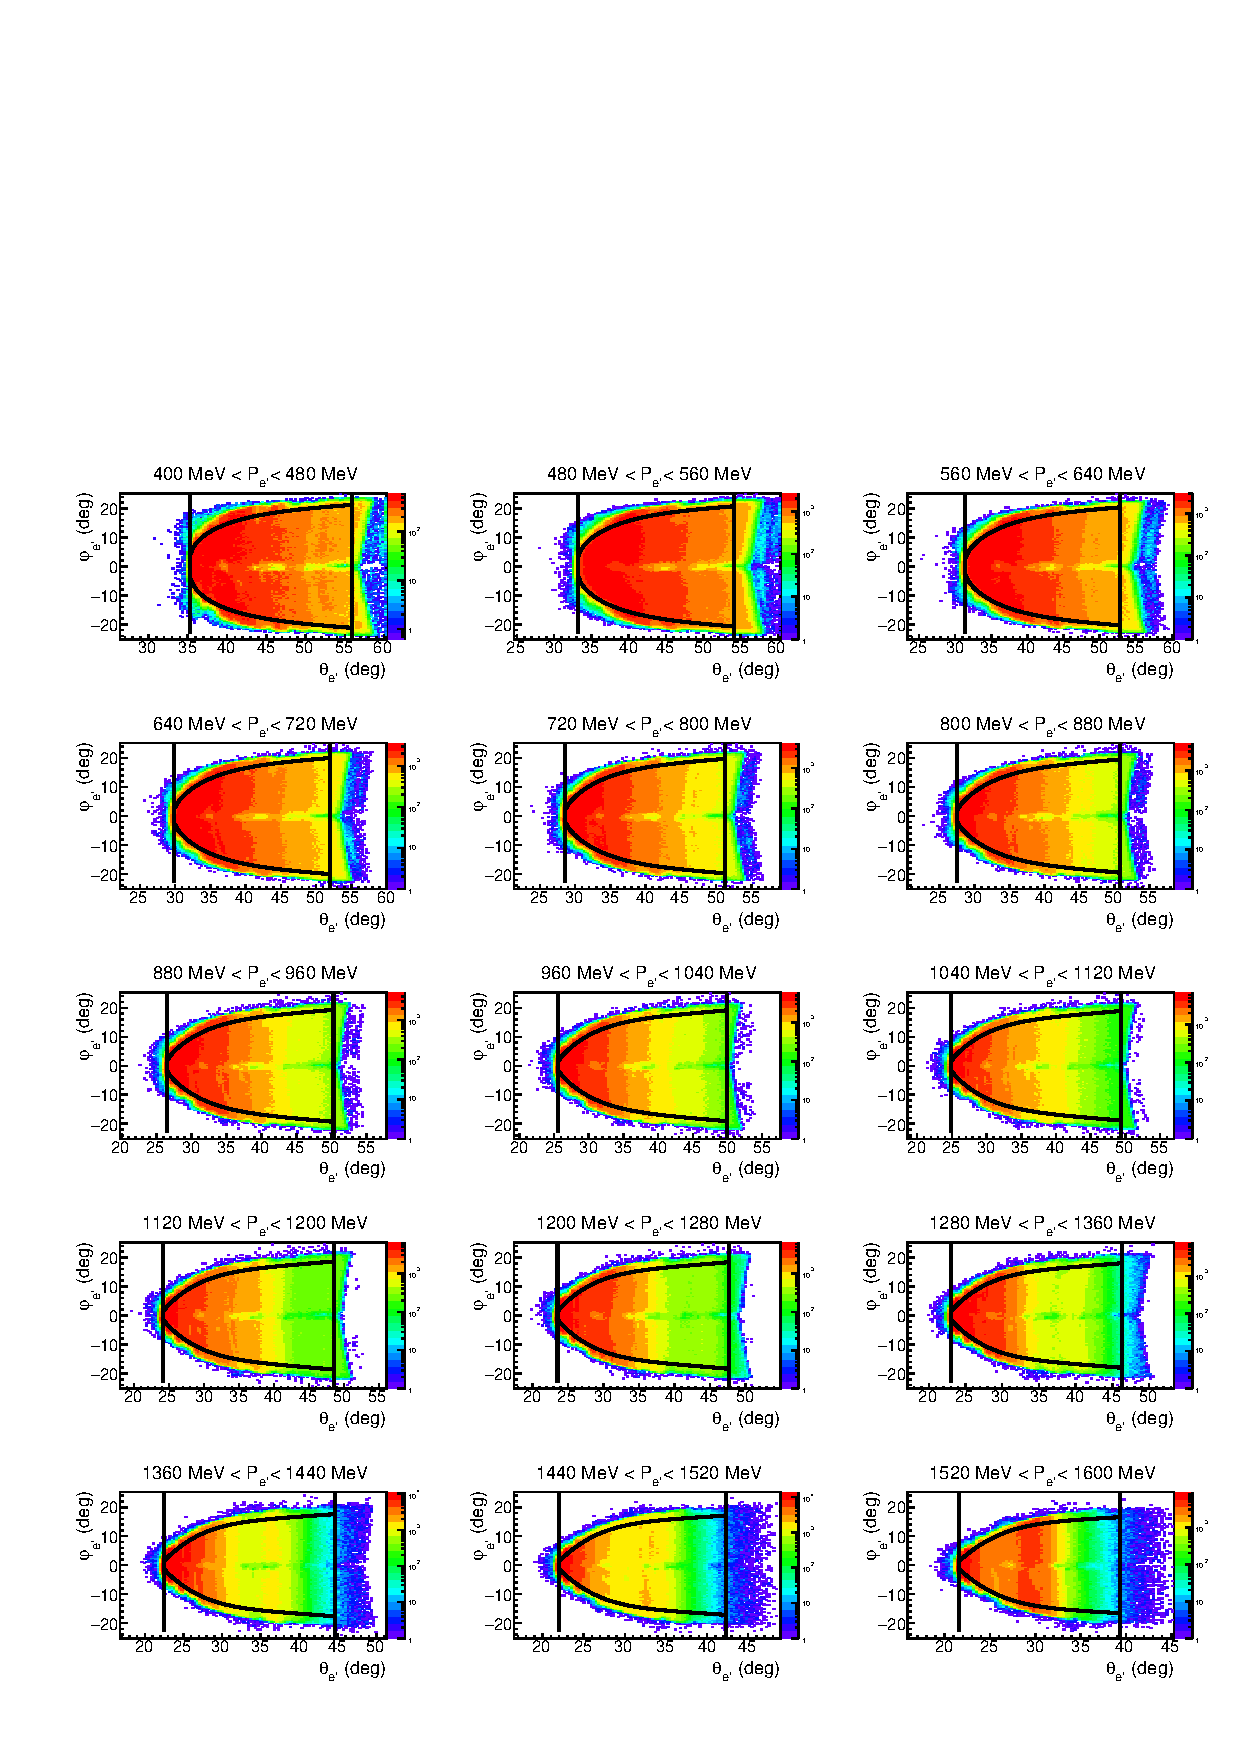
\includegraphics[width=\textwidth]{pictures/other_cuts/fiducial/el_fid_2dim_mom_slice_fin.pdf}}
\caption{\small $\varphi$ versus $\theta$ distributions for electron candidates for different 80-MeV-wide momentum slices plotted for events from all CLAS sectors. Curves show the applied fiducial cuts, vertical lines stand for $\theta_{e'}^{min}$ and $\theta_{e'}^{max}$. The angles are taken at the interaction vertex. For each momentum slice the shape of the fiducial cut was calculated for the value of the electron momentum taken in the center of the momentum bin.  \label{fig:fiduch_el_2d}}
\end{center}
\end{figure}

\clearpage

\begin{figure}[htp]
\begin{center}
\framebox{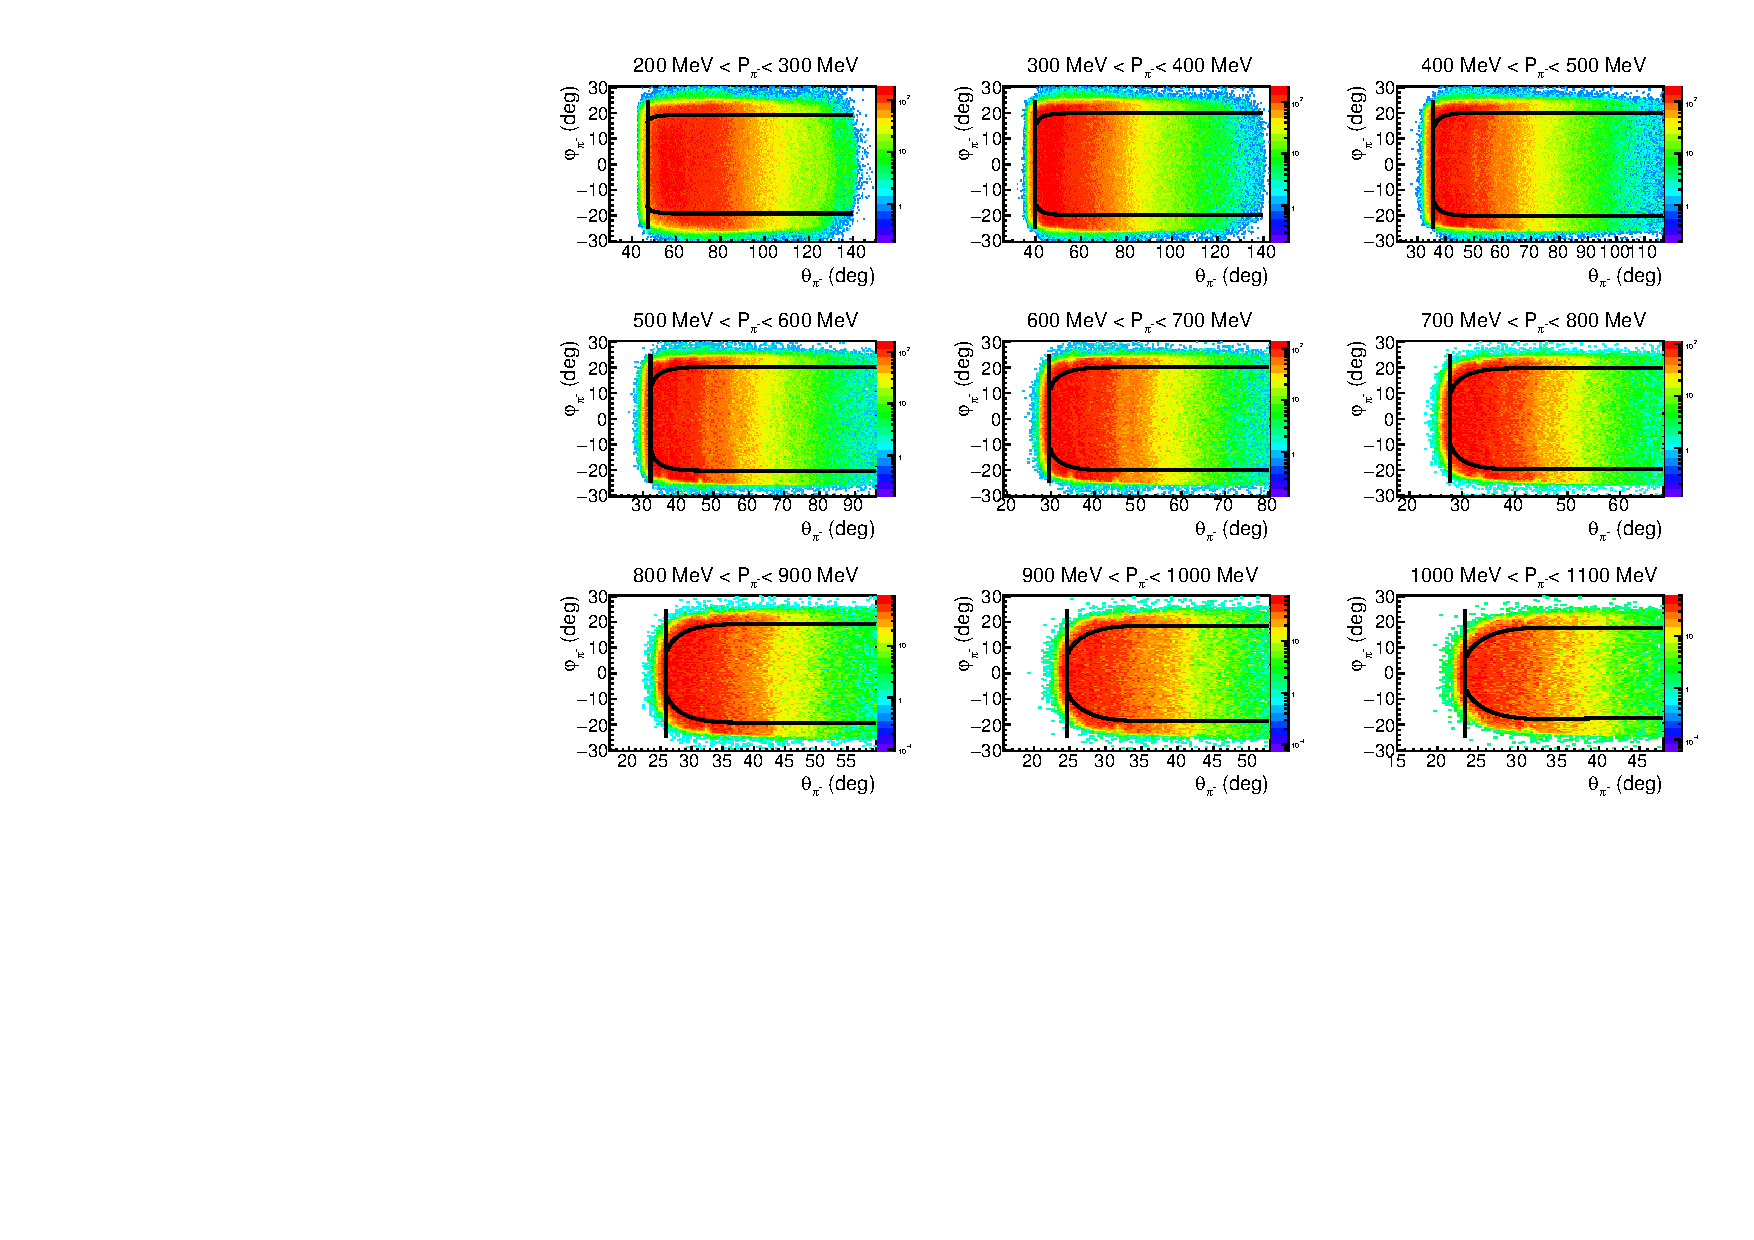
\includegraphics[width=\textwidth]{pictures/other_cuts/fiducial/pim_fid_2dim_mom_slice.pdf}}
\caption{\small $\varphi$ versus $\theta$ distributions for negative pion candidates for different 100-MeV-wide momentum slices plotted for events from all CLAS sectors. Curves show the applied fiducial cuts, vertical lines stand for $\theta_{\pi}^{min}$ and $\theta_{\pi}^{max}$. The angles are taken at the interaction vertex. For each momentum slice the shape of the fiducial cut was calculated for the value of the pion momentum taken in the center of the momentum bin. \label{fig:fiduch_pim_2d}}
\end{center}
\end{figure}


The fiducial cut for electron candidates is illustrated in Fig.~\ref{fig:fiduch_el_2d}, where the cut curves are superimposed on the $\varphi$ versus $\theta$ distributions for different 80-MeV-wide momentum slices. Vertical lines correspond to $\theta_{e'}^{min}$ and $\theta_{e'}^{max}$. For each momentum slice the shape of the fiducial cut was calculated for the value of the electron momentum taken in the center of the momentum bin. The depleted area around $\varphi_{e'} = 0$ corresponds to the inefficient region in CC and was discussed above in Sect.~\ref{Sect:cc_cuts}.  

The fiducial cut for negative pion candidates is illustrated in Fig.~\ref{fig:fiduch_pim_2d}, where the cut curves are superimposed on the $\varphi$ versus $\theta$ distributions for different 100-MeV-wide momentum slices. Vertical lines correspond to $\theta_{\pi}^{min}$ and $\theta_{\pi}^{max}$. For each momentum slice the shape of the fiducial cut was calculated for the value of the pion momentum taken in the center of the momentum bin.

The same fiducial cuts for negatively charged particles are also applied to the reconstructed Monte Carlo events.
%\clearpage

\begin{figure}[htp]
\begin{center}
\framebox{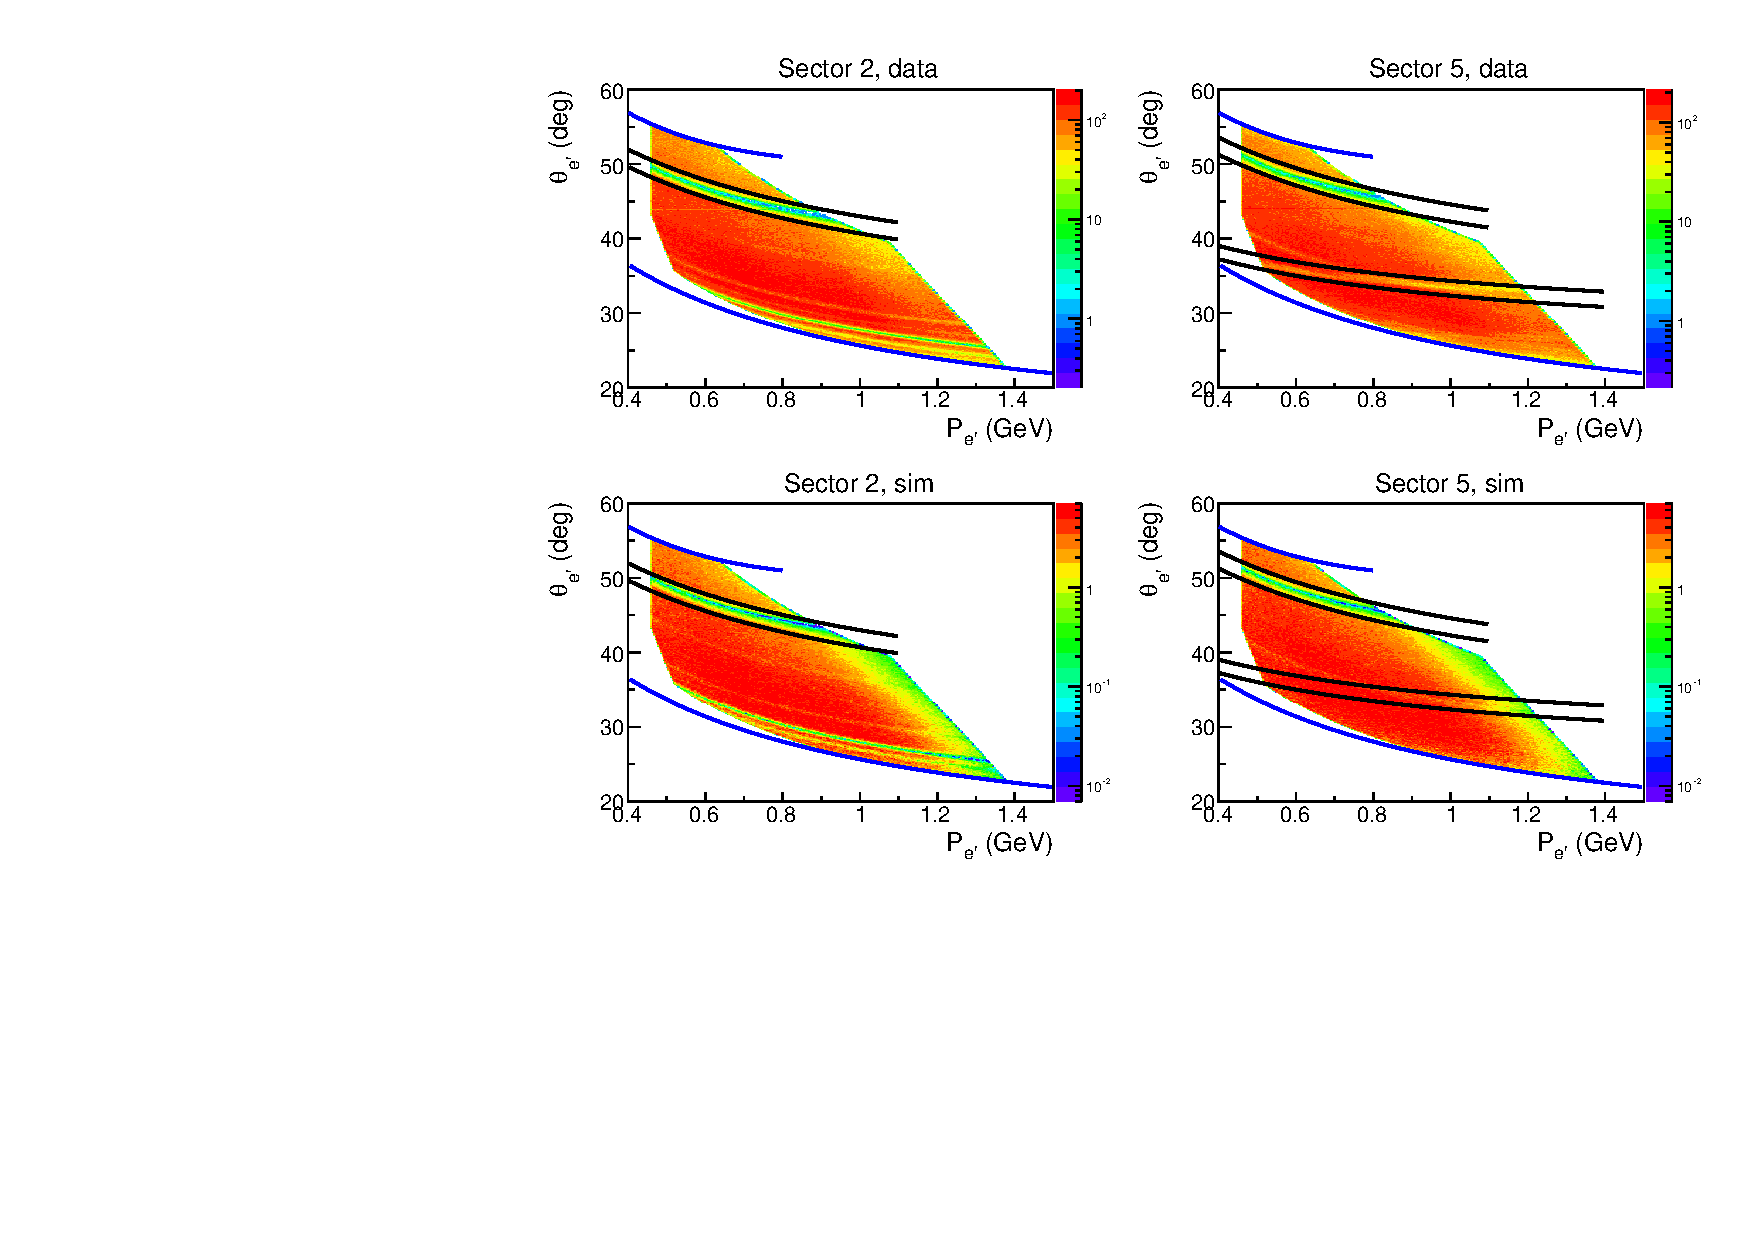
\includegraphics[width=9.cm]{pictures/other_cuts/fiducial/th_vs_p_el_new.pdf}}
\caption{\small  $\theta$ versus momentum distributions for electron candidates for CLAS sectors two (left side) and five (right side). The angle $\theta$ is taken at the interaction vertex. Top row corresponds to the data, bottom row corresponds to the reconstructed Monte Carlo events. Blue curves correspond to $\theta_{e'}^{min}$ and $\theta_{e'}^{max}$. Black curves correspond to additional fiducial $\theta$ versus momentum cuts. These distributions are plotted under the conditions 1.3~GeV $< W <$ 1.825~GeV and 0.4~GeV$^{2}$ $< Q^{2} <$ 1.0~GeV$^{2}$ which account for the extra cuts of the distribution edges. Other small inefficiencies that are seen in these plots are due to the geometrical cut in the CC plane (see Sect.~\ref{Sect:cc_cuts}). \label{fig:th_vs_p_el}}
\end{center}
\end{figure}

There are some additional dead areas in CLAS acceptance that are not related to the gaps between the sectors and limitations on the detection polar angle. They are typically caused by some inefficiencies in the Drift Chambers and Time-of-Flight system (dead wires or PMTs). Some of them are well reproduced in the Monte Carlo simulation, while others are not. To exclude the latter from the analysis and to eliminate events near the acceptance edges, additional fiducial cuts on $\theta$ versus momentum distributions are applied. These cuts are individual for each CLAS sector. They are shown by the black curves for real and Monte Carlo events in Fig.~\ref{fig:th_vs_p_el} for electron candidates and in Fig.~\ref{fig:th_vs_p_pim} for negative pion candidates. 

\begin{figure}[htp]
\begin{center}
\framebox{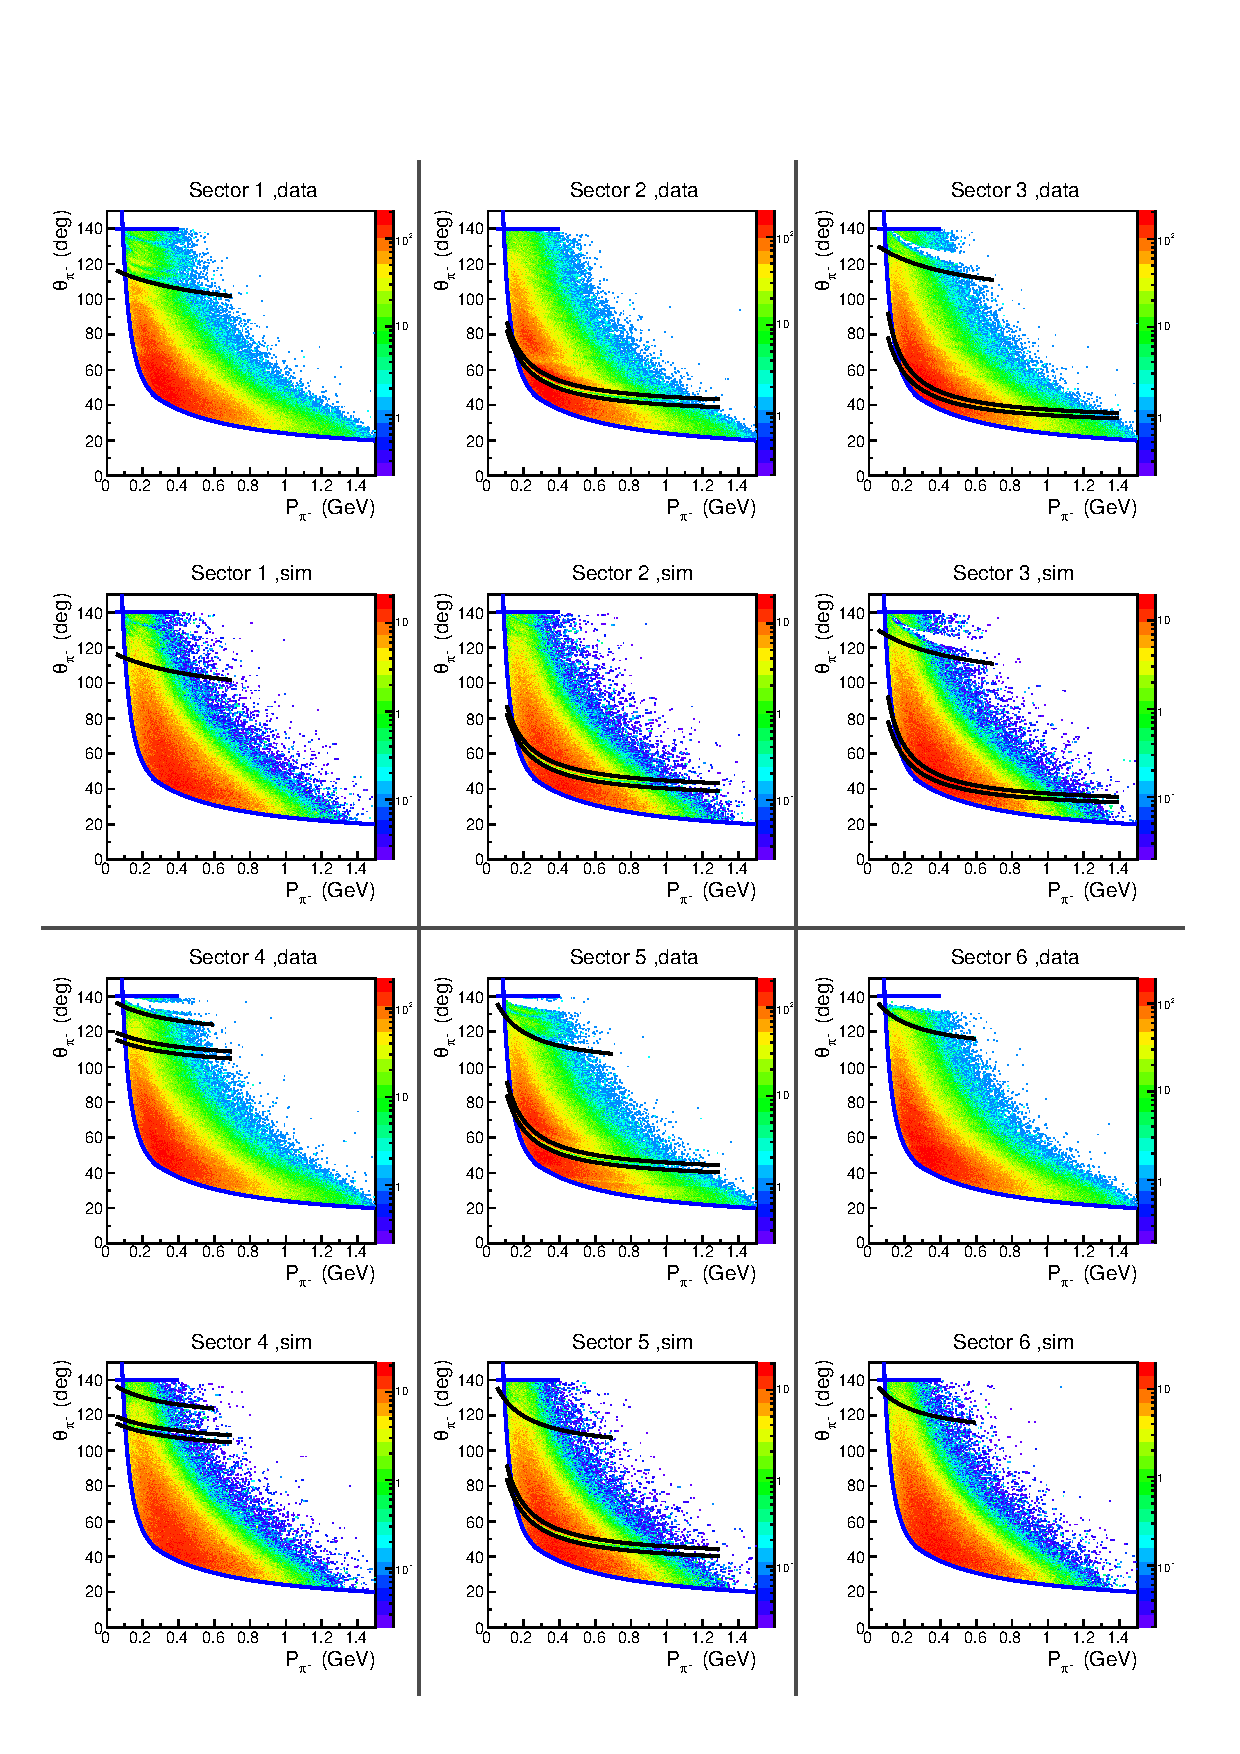
\includegraphics[width=14.5cm]{pictures/other_cuts/fiducial/th_vs_p_pim2.pdf}}
\caption{\small $\theta$ versus momentum distributions for negative pion candidates for different CLAS sectors. The angle $\theta$ is taken at the interaction vertex. Plots are given both for real data and reconstructed Monte Carlo events. Blue curves correspond to $\theta_{\pi}^{min}$ and $\theta_{\pi}^{max}$. Black curves correspond to additional fiducial $\theta$ versus momentum cuts. \label{fig:th_vs_p_pim}}
\end{center}
\end{figure}
\clearpage

For the electron distributions shown in Fig.~\ref{fig:th_vs_p_el} inefficient areas in sectors two and five correspond to bad TOF paddles \#16 and \#17, respectively. Other small inefficiencies that are seen in these plots are due to the geometrical cut in the CC plane (see Sect.~\ref{Sect:cc_cuts}), they are almost identical for data and Monte Carlo events and, therefore, no additional fiducial cuts are needed for them.  $\theta$ versus momentum distributions for electron candidates in other sectors do not show significant inefficiencies. 

\subsubsection{Fiducial cuts for positively charged particles}
\label{Sect:fiduc_pos}

For positively charged particles, which are outbending in the ``e1e" experiment, momentum independent and symmetrical fiducial cuts suit our purpose best. The analytical shapes of these cuts can be found in Ref.~\cite{my_an_note:2020}. They were also taken from the analysis~\cite{Fed_an_note:2017} and carefully adjusted to the data. %All angles in Eq.~\eqref{eq:fiduch_pos} are taken at the interaction vertex and assumed to be in degrees. Events that satisfy the criteria $\theta^{min} < \theta < \theta^{max}$ and $\varphi^{min} < \varphi < \varphi^{max}$ are selected for the analysis. 


\everypar{\looseness=-1}
Fiducial cuts for positive hadron candidates are illustrated in Fig.~\ref{fig:fiduch_pos_2d}, where the cut curves are superimposed on the $\varphi$ versus $\theta$ distributions for protons (left) and pions (right). Vertical lines correspond to $\theta^{min}$ and $\theta^{max}$. Additional fiducial cuts in $\theta$ versus momentum coordinates are shown in Fig.~\ref{fig:th_vs_p_pr} for protons and in Fig.~\ref{fig:th_vs_p_pip} for $\pi^{+}$. The same fiducial cuts for positively charged particles are also applied to the reconstructed Monte Carlo events.
\begin{figure}[!ht]
\begin{center}
\framebox{
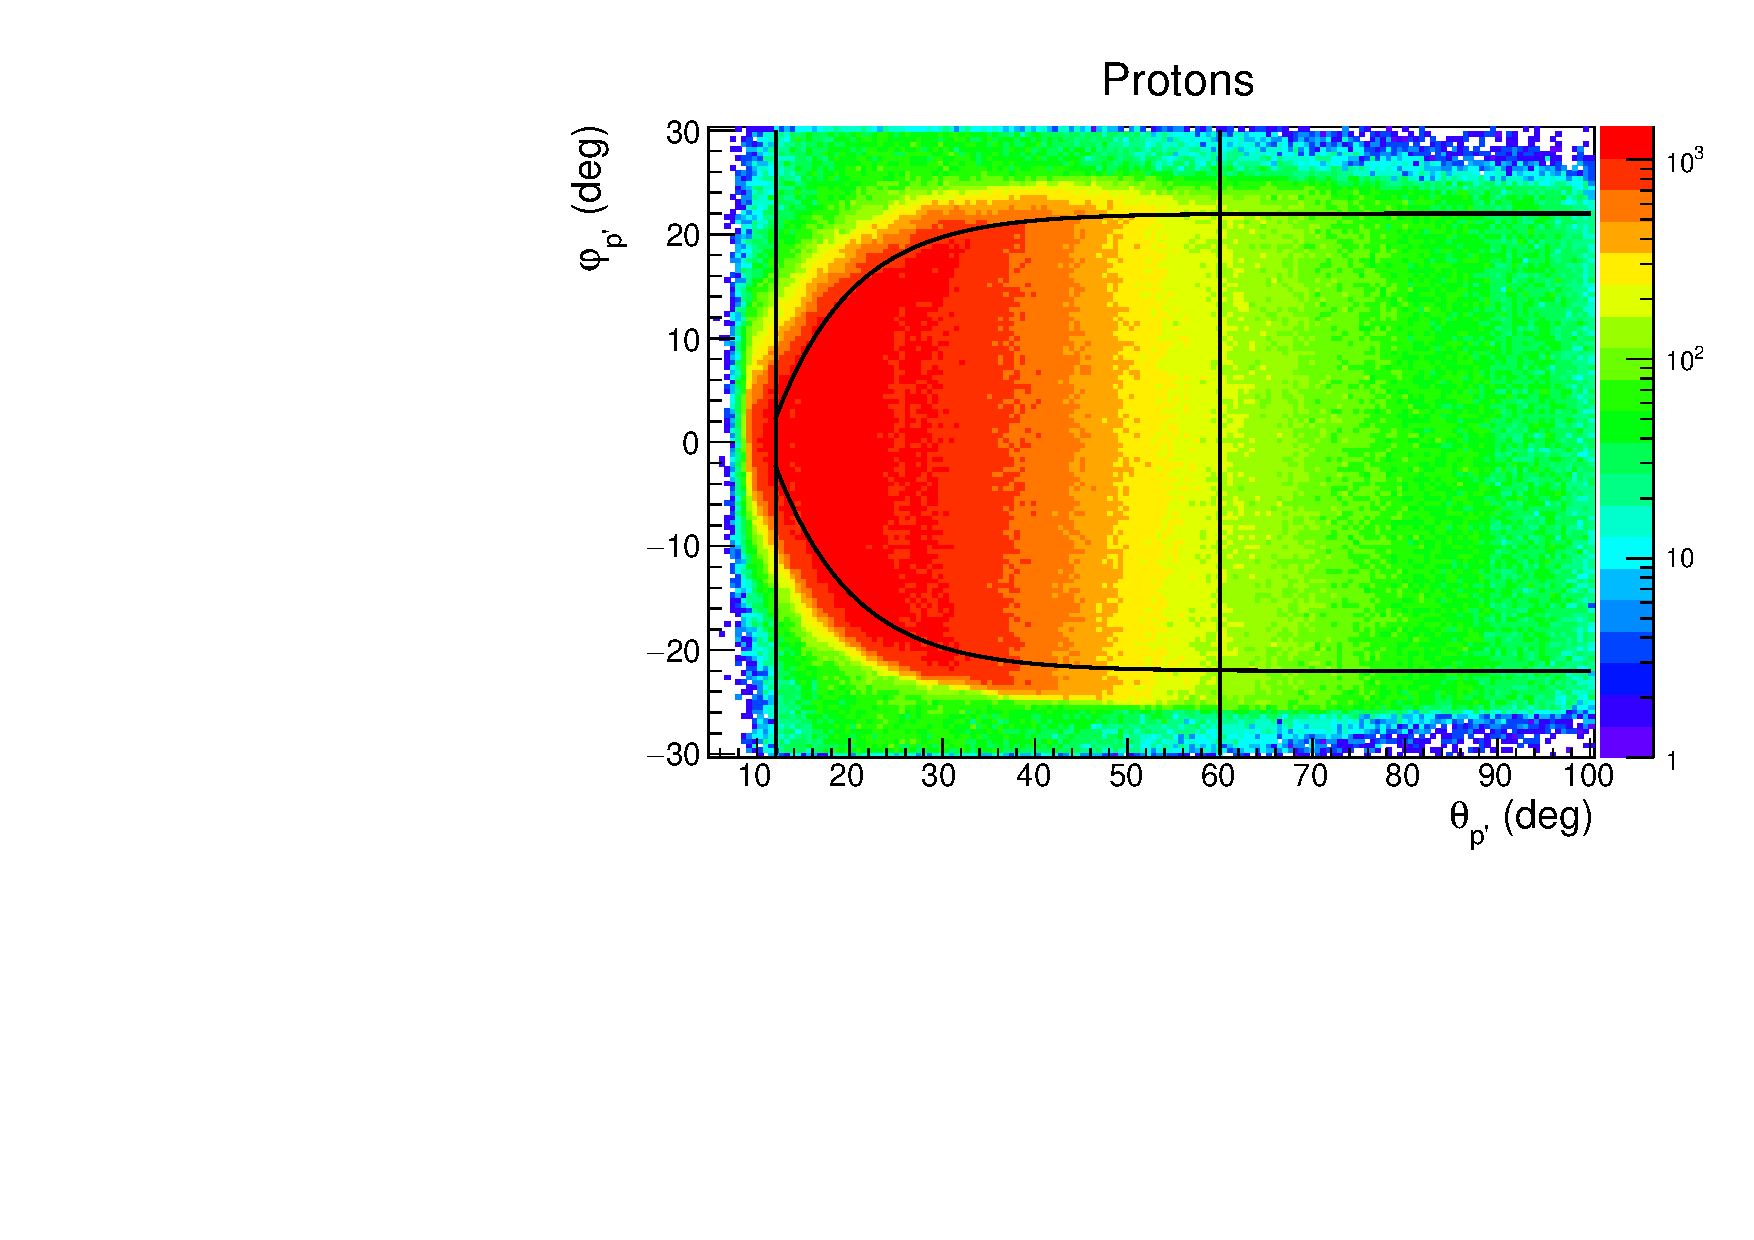
\includegraphics[width=0.4\textwidth]{pictures/other_cuts/fiducial/fid_p_2dim.pdf}
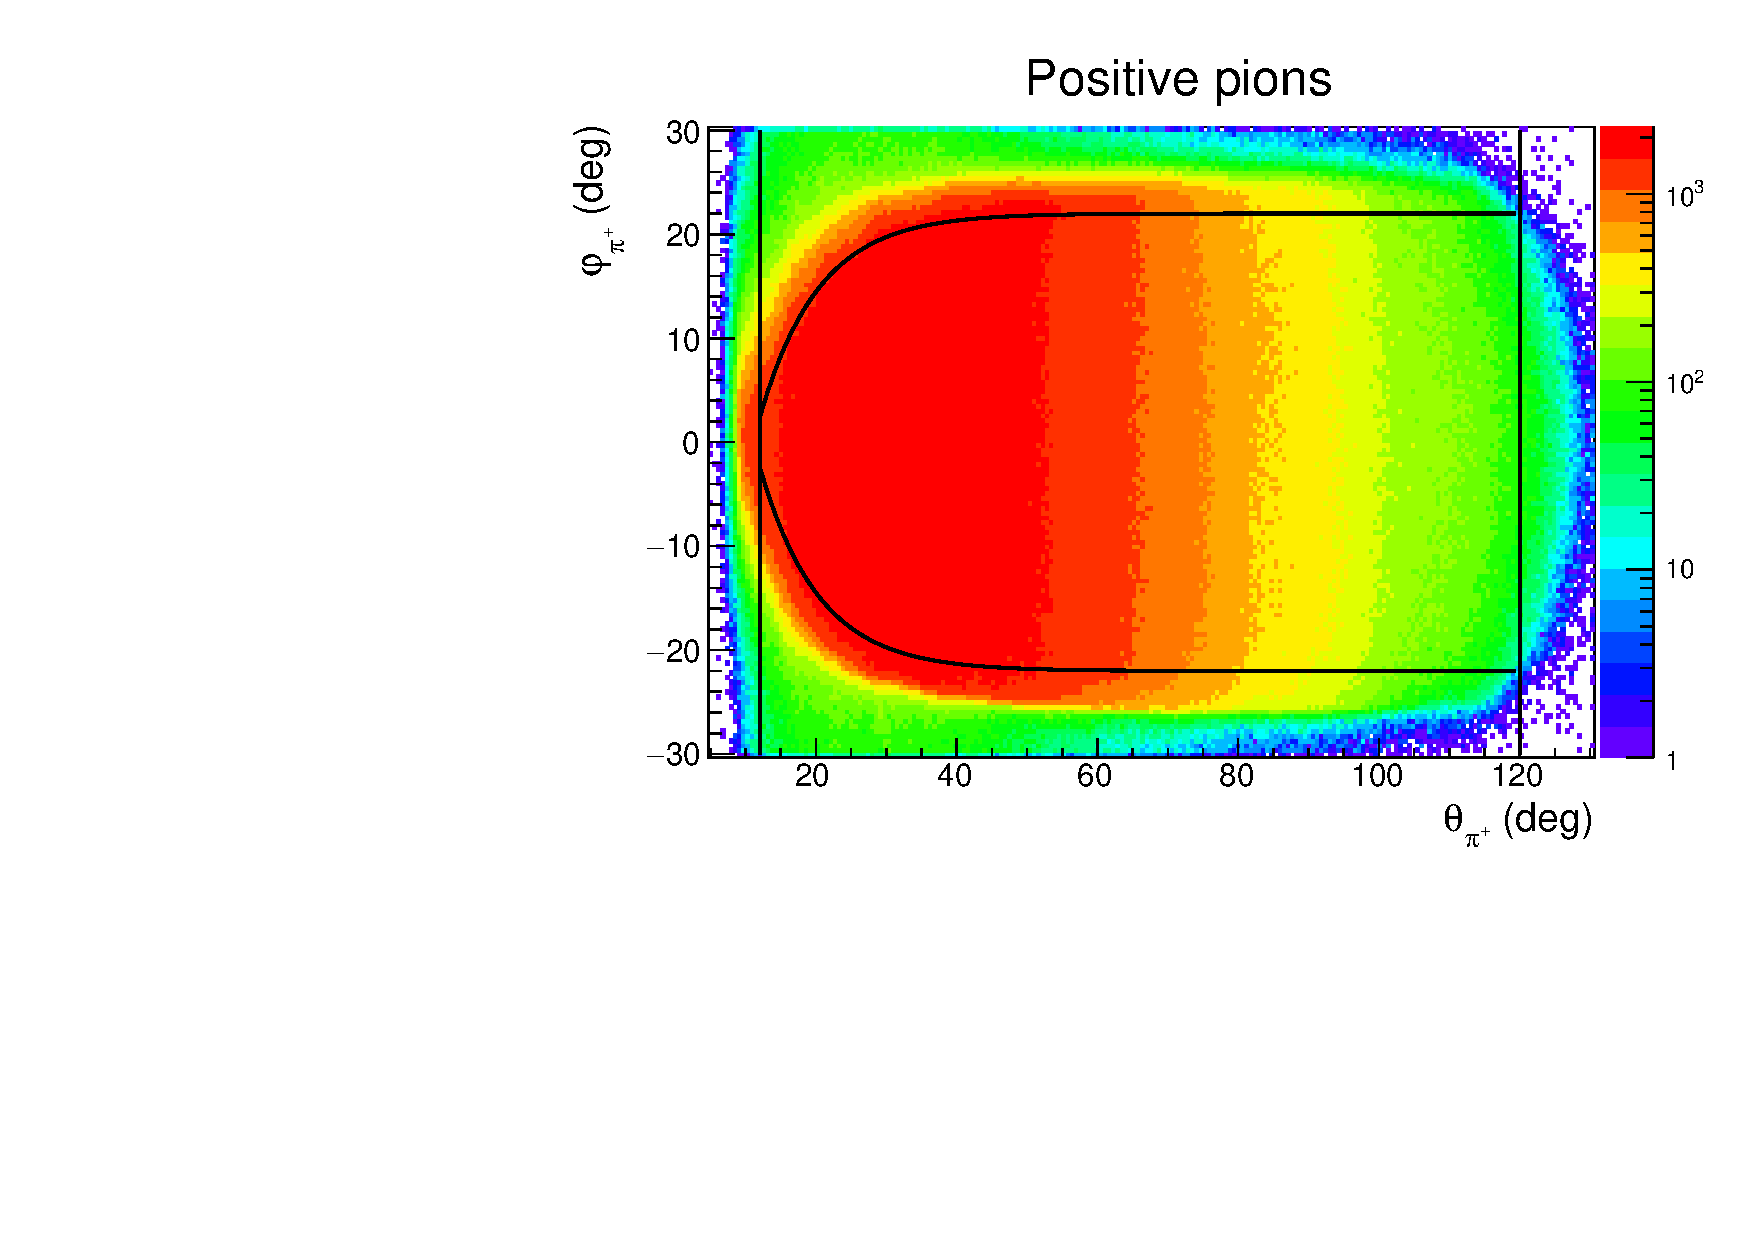
\includegraphics[width=0.4\textwidth]{pictures/other_cuts/fiducial/fid_pip_2dim.pdf}}
\end{center}
\caption{\small $\varphi$ versus $\theta$ distributions for positive hadron candidates: left plot -- for protons, right plot -- for positive pions. The distributions are plotted for all CLAS sectors. Curves show the applied fiducial cuts, vertical lines stand for $\theta^{min}$ and $\theta^{max}$. The angles are taken at the interaction vertex.}
\label{fig:fiduch_pos_2d}
\end{figure}


%\clearpage

\begin{figure}[htp]
\begin{center}
\framebox{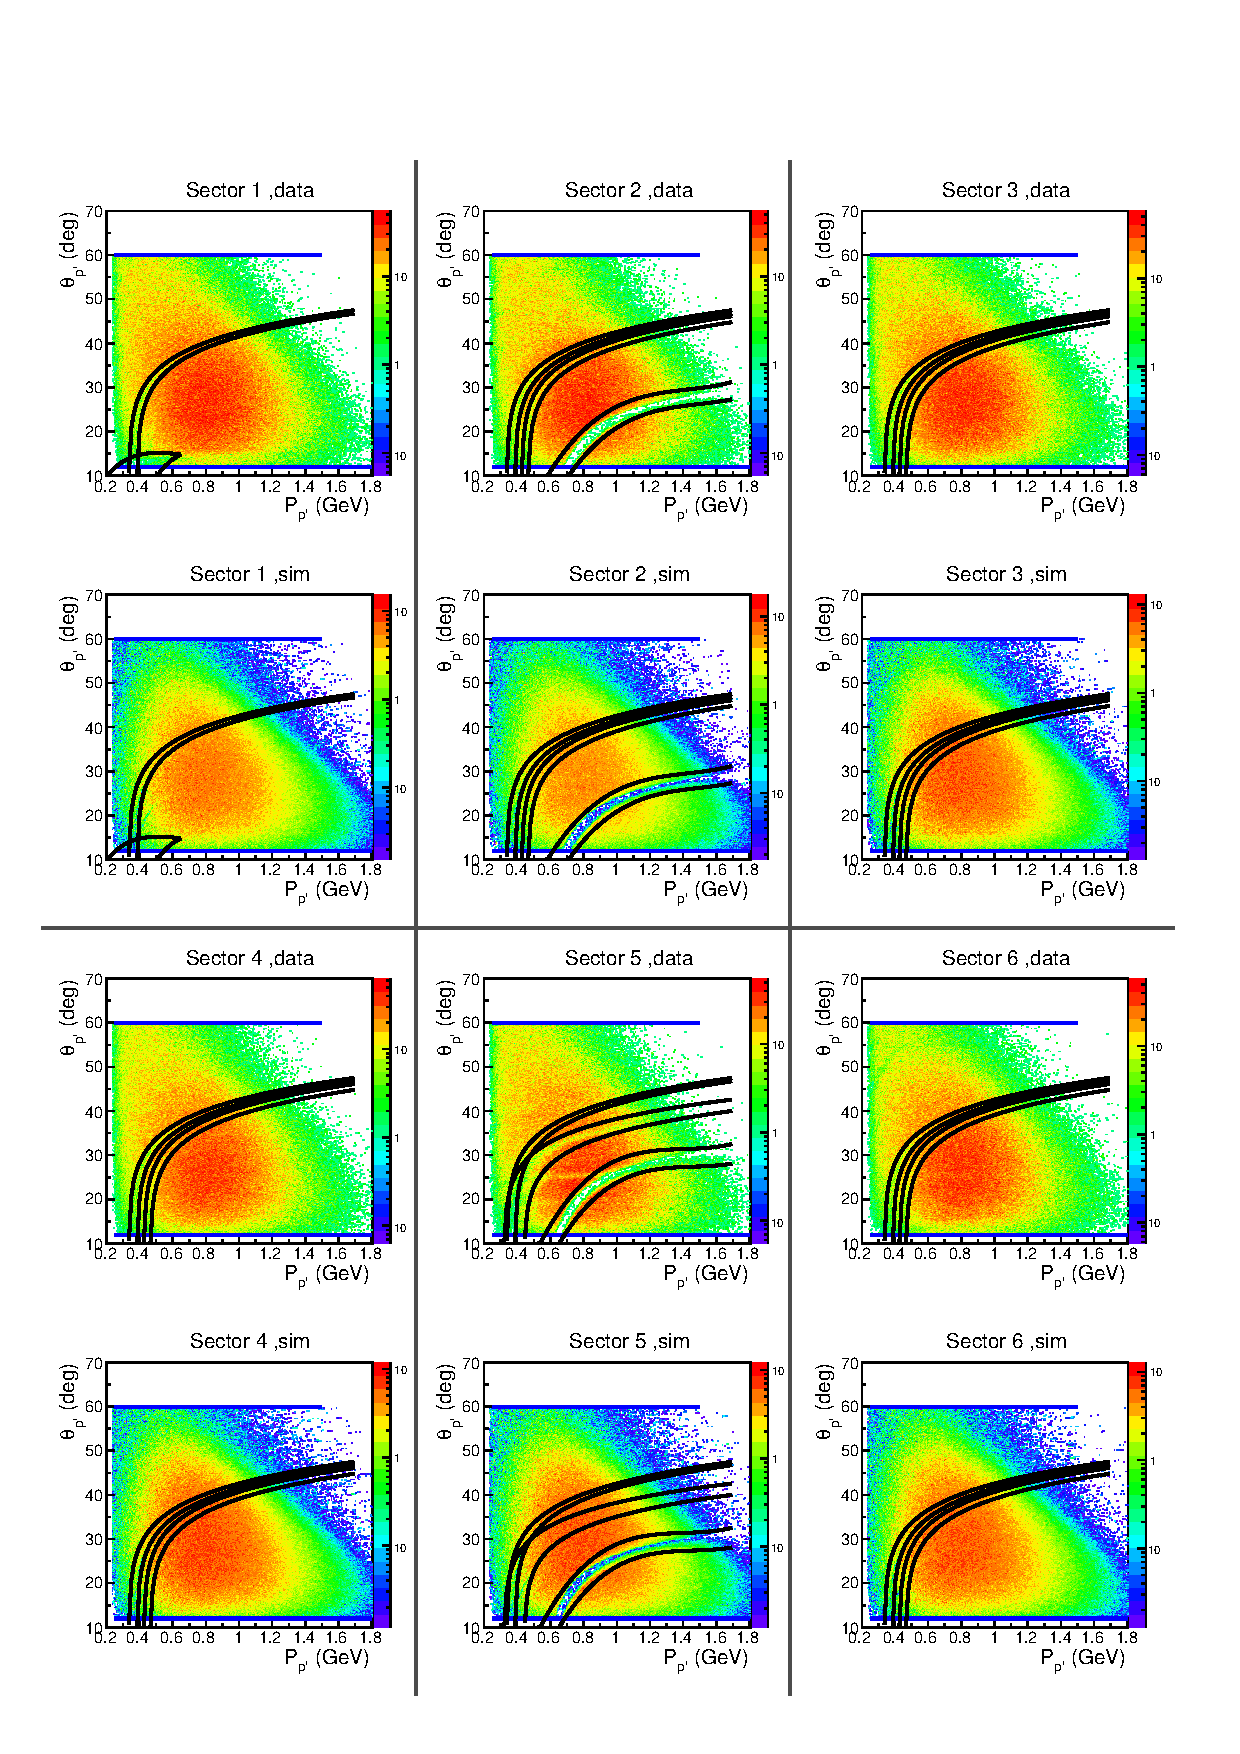
\includegraphics[width=14.5cm]{pictures/other_cuts/fiducial/th_vs_p_pr.pdf}}
\caption{\small $\theta$ versus momentum distributions for proton candidates for different CLAS sectors. The angle $\theta$ is taken at the interaction vertex. Plots are given both for the real data and reconstructed Monte Carlo events. Blue lines correspond to $\theta^{min}$ and $\theta^{max}$. Black curves correspond to additional fiducial $\theta$ versus momentum cuts. \label{fig:th_vs_p_pr}}
\end{center}
\end{figure}

\clearpage

\begin{figure}[htp]
\begin{center}
\framebox{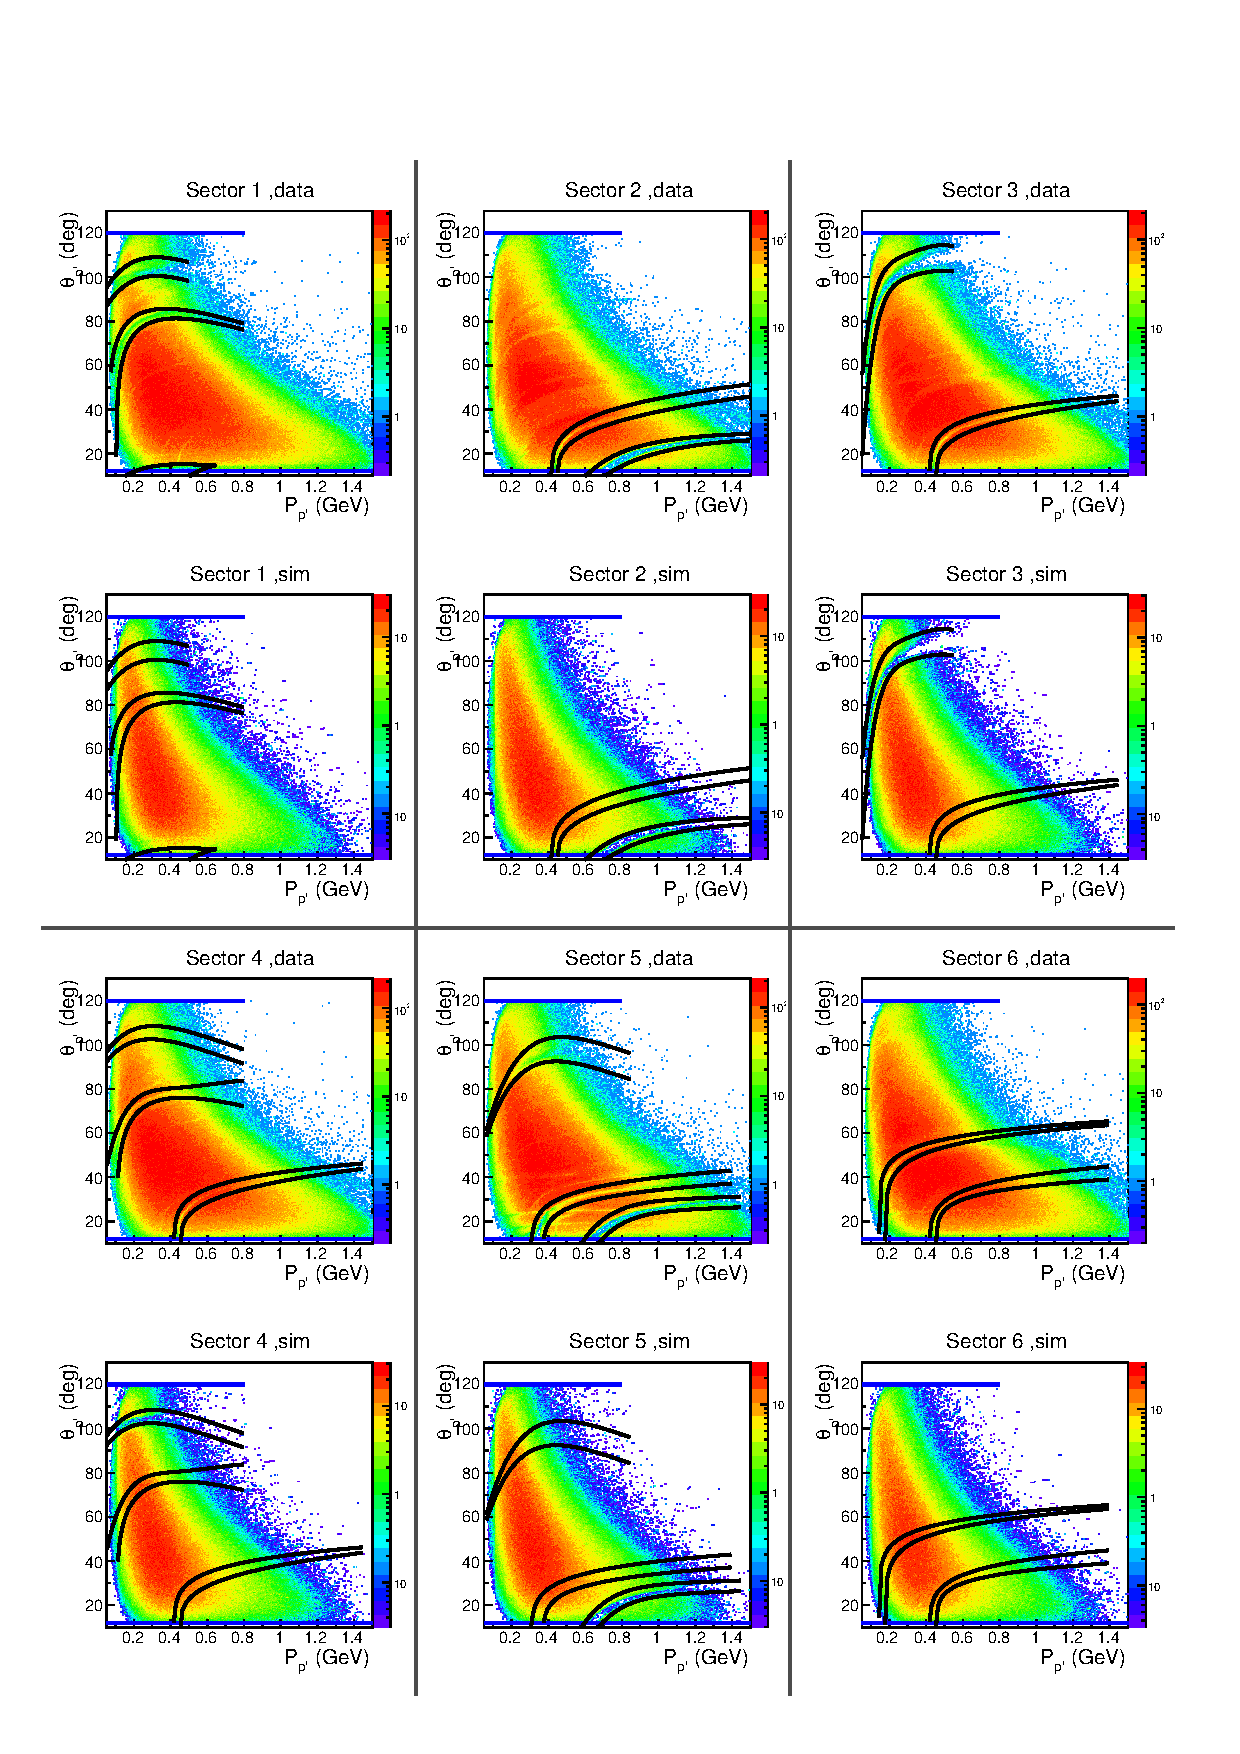
\includegraphics[width=14.5cm]{pictures/other_cuts/fiducial/th_vs_p_pip.pdf}}
\caption{\small $\theta$ versus momentum distributions for positive pion candidates for different CLAS sectors. The angle $\theta$ is taken at the interaction vertex. Plots are given both for the real data and reconstructed Monte Carlo events. Blue lines correspond to $\theta^{min}$ and $\theta^{max}$. Black curves correspond to additional fiducial $\theta$ versus momentum cuts. \label{fig:th_vs_p_pip}}
\end{center}
\end{figure}

\clearpage

\subsection{Data quality check}
\label{Sect:qcheck}
\afterpage{\clearpage}

During a long experimental run, variations of the experimental conditions, e.g. fluctuations in the target density, deviations of the beam current and position as well as changes in the response of parts of the detector, can lead to fluctuations in event yields. Only the parts of the run with relatively stable event rates are selected for the analysis.
Therefore, cuts on Data Acquisition (DAQ) live time and number of events per Faraday cup (FC) charge need to be established.
%\footnote[1]{This quality check cuts are used only for the full target runs}. 

\afterpage{\clearpage}
\begin{figure}[htp]
\begin{center}
\framebox{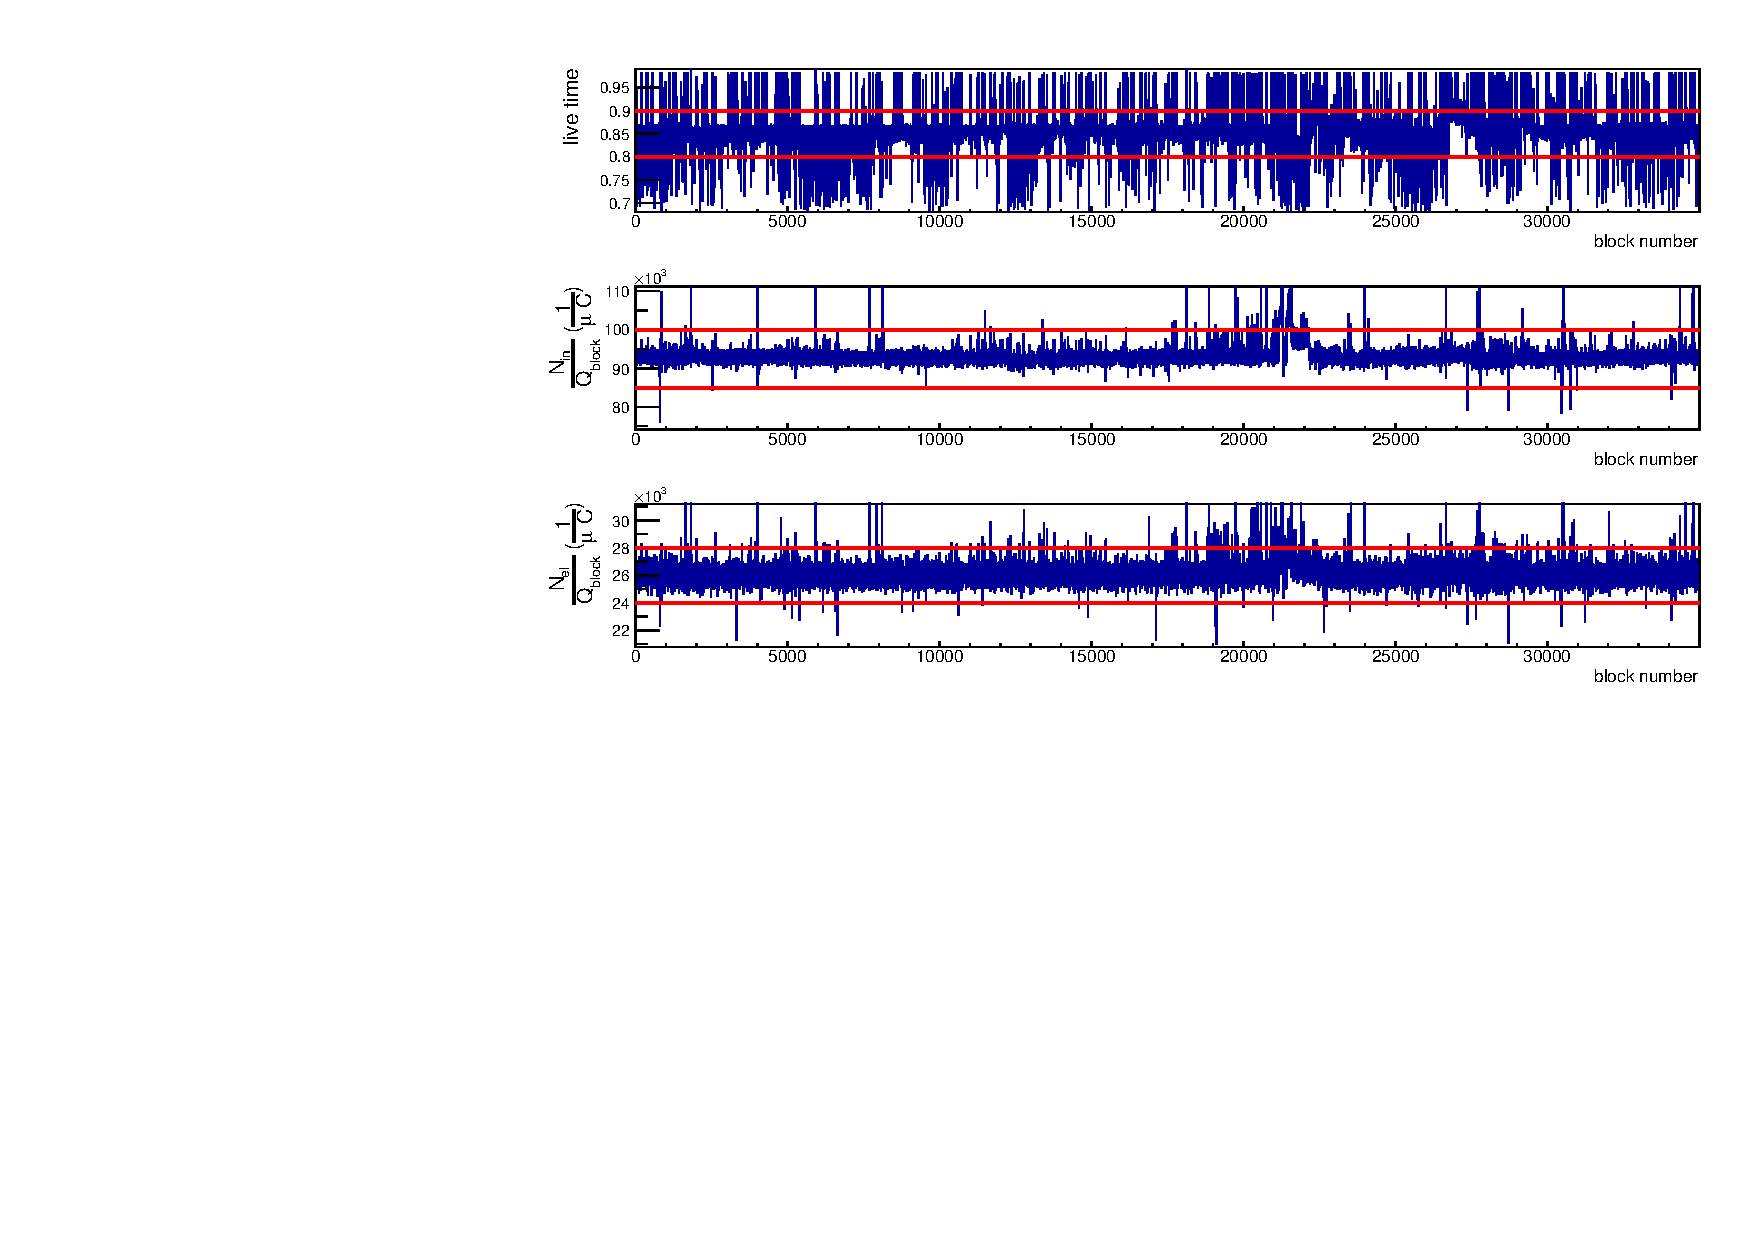
\includegraphics[width=\textwidth]{pictures/other_cuts/qual_check/livetime_incl_elast_2d_norebin.pdf}}
\caption{\small In the top plot DAQ live time is shown as a function of {\em block} number. Each {\em block} corresponds to  the portion of events that is accumulated during a single Faraday cup charge reading cycle. {\em Block} numbers range from one to the maximum number and represent the run duration in the units of Faraday cup readouts. In the middle plot the number of inclusive events accumulated within each {\em block} divided by FC charge accumulated during the {\em block} is  plotted versus {\em block} number. The bottom plot shows the number of elastic events accumulated within each {\em block} divided by FC charge accumulated during the {\em block} as a function of {\em block} number. Horizontal red lines show the applied cuts.  \label{fig:qual_check_2d}}
\end{center}
\end{figure}\vspace{-0.75em}

The FC charge updates with a given frequency, so the whole run time can be divided into so-called {\em blocks}. Each {\em block} corresponds to the portion of time between two FC charge readouts. FC charge readouts happen approximately once every ten seconds. The {\em block} number ranges over the run time from one to a certain maximum number. The first and last {\em blocks} in each run file are excluded from the analysis, since FC readout is not synchronized in time with the start/stop of writing to the file.


The DAQ live time is the portion of time within the {\em block} during which the DAQ system is able to accumulate events. A significant deviation of the live time from the average value indicates event rate alteration. For instance, if the live time is close to one, then the event rate is too low and vice versa.
In Fig.~\ref{fig:qual_check_2d} the DAQ live time (top plot) as well as the yields of inclusive (middle plot) and elastic (bottom plot) events normalized to FC charge are shown as a function of {\em block} number. {\em Blocks} between the horizontal red lines in Fig.~\ref{fig:qual_check_2d} are selected for the analysis.
Due to the enormous amount of {\em blocks} all of them cannot be made visible in two-dimensional histograms, therefore, to have a general feeling of what amount of blocks are removed, the $y$-axis projections of the histograms in Fig.~\ref{fig:qual_check_2d} are given in Fig.~\ref{fig:qual_check_1d}. The horizontal red cut lines in Fig.~\ref{fig:qual_check_2d} correspond to the vertical red cut lines in Fig.~\ref{fig:qual_check_1d}.

\afterpage{\clearpage}
\begin{figure}[htp]
\begin{center}
\framebox{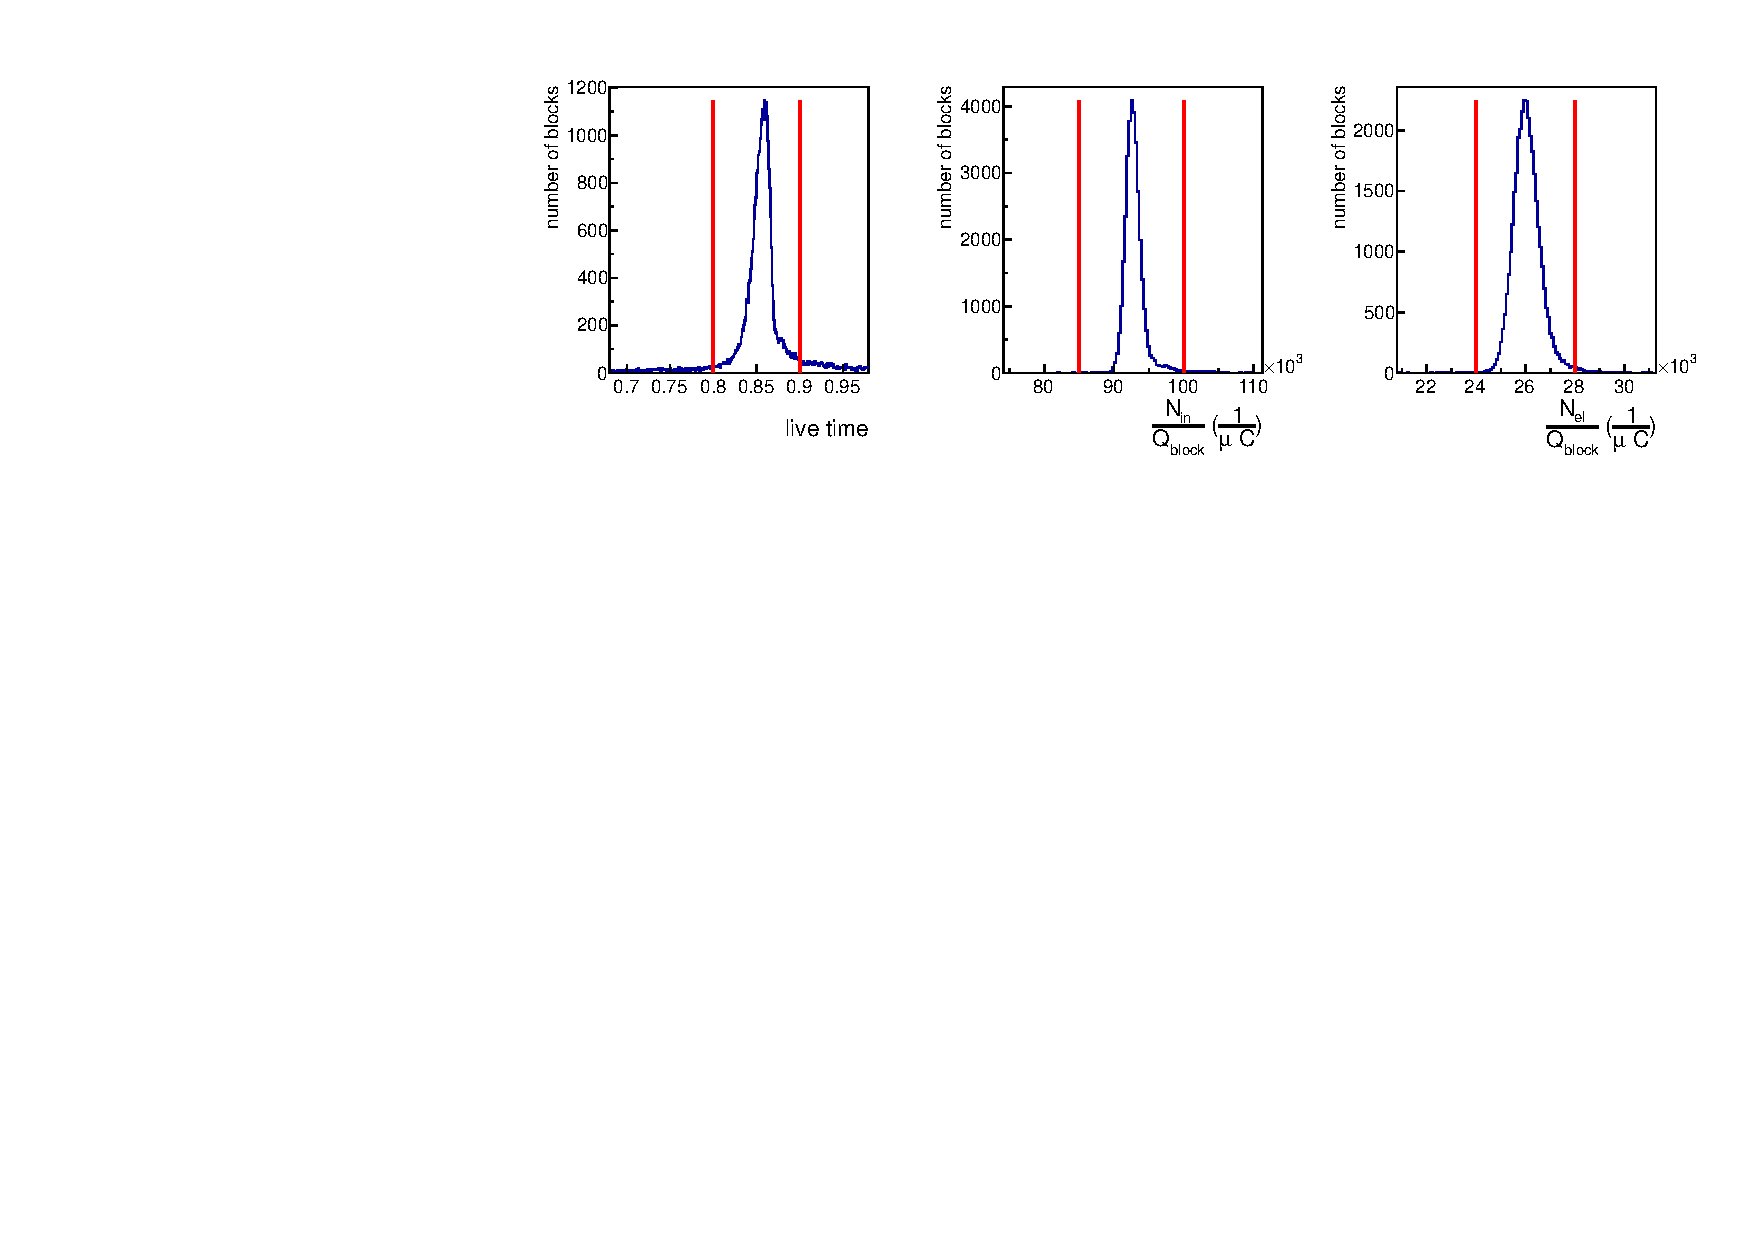
\includegraphics[width=\textwidth]{pictures/other_cuts/qual_check/livetime_incl_elast_1d.pdf}}
\caption{\small Number of {\em block} occurrences (see explanation in the text) as a function of DAQ live time (left plot), inclusive event yield normalized to FC charge  (middle plot), and  elastic event yield normalized to FC charge (right plot). The vertical red cut lines correspond to the horizontal red cut lines in Fig.~\ref{fig:qual_check_2d}. \label{fig:qual_check_1d}}
\end{center}
\end{figure}



\subsection{Vertex cut}
\label{Sect:vertex}
\afterpage{\clearpage}


In Fig.~\ref{fig:z_el_full_empty} distributions of electron $z$-coordinate at the interaction vertex are shown for events from both empty and full target runs for all six CLAS sectors. The vertical red lines show the cut that is applied in addition to the empty target event subtraction. The vertical dashed line marks the position $z = -0.4$~cm, where the center of the target is expected to be. However, as seen in Fig.~\ref{fig:z_el_full_empty}, the $z_{e'}$ distributions demonstrate small sector dependent deviations from their expected position. The source of these deviations is an offset of the beam position from the CLAS central line $(x, y) = (0, 0)$. 

\begin{figure}[!ht]
\begin{center}
\framebox{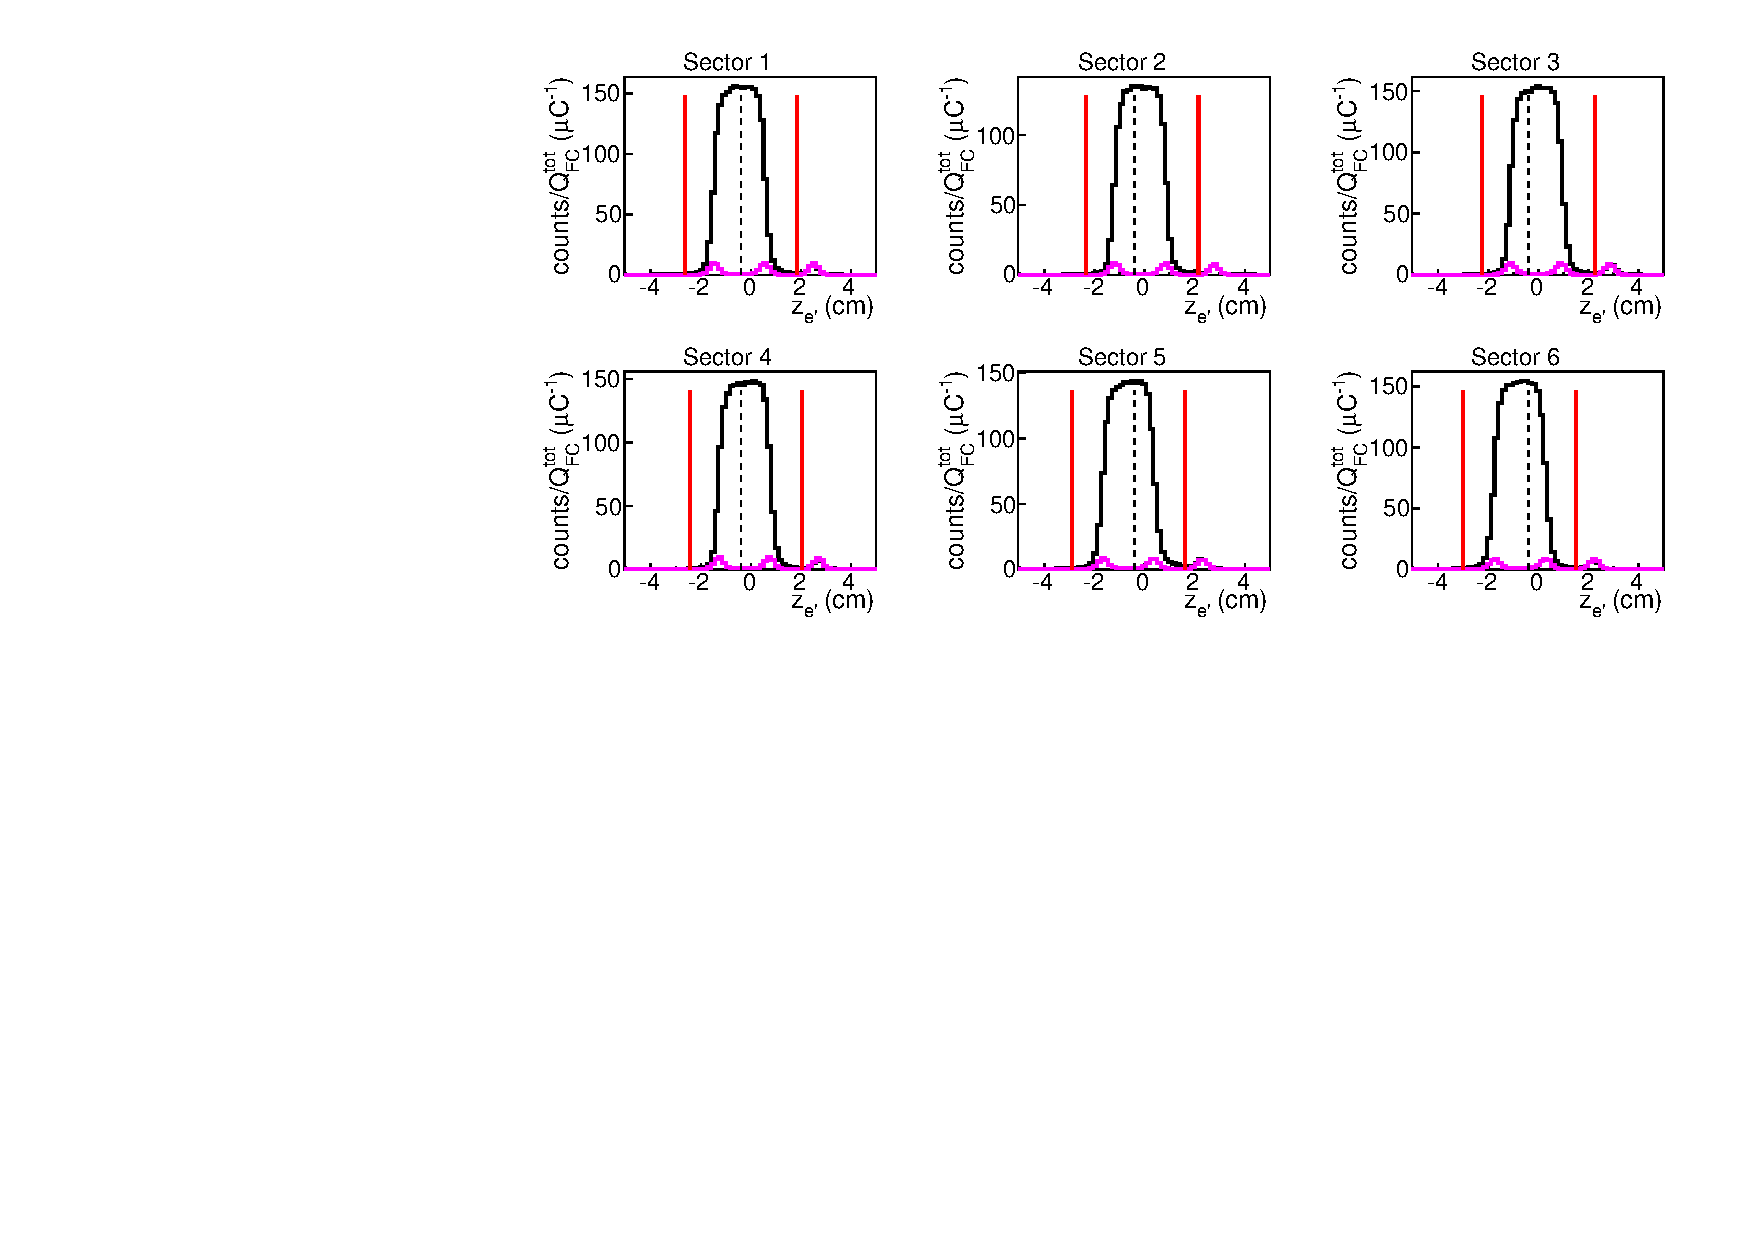
\includegraphics[width=13.1cm]{pictures/other_cuts/z_vertex/z_el_full_empty3.pdf}}
\end{center}
\caption{\small Distributions of the electron $z$-coordinate at the vertex for full (black curves) and empty (magenta curves) target runs for the six CLAS sectors. Vertical dashed lines mark the position $z = -0.4$~cm, where the center of the target is expected to be. Vertical red lines show the applied cuts. Both full and empty target distributions are normalized to the corresponding FC charge. }
\label{fig:z_el_full_empty}
\end{figure}

To estimate the beam offset, the $y_{e'}^{dc}$ versus $x_{e'}^{dc}$ distribution was investigated, where $x_{e'}^{dc}$ and $y_{e'}^{dc}$ are the corresponding coordinates of an electron at the point of interaction, which are taken from the DCPB bank (variables $\rm X\_v$ and $\rm Y\_v$, respectively). This distribution is shown in Fig.~\ref{fig:beam_offset}, where the intersections of black dashed and solid red lines indicate the nominal and actual beam positions, respectively. The actual beam position was found to be ($x$,~$y$) = (0.057~cm,~-0.182~cm). The generated Monte Carlo events were reconstructed taking into account the determined beam offset to improve resemblance to the real data\footnote[6]{The following option was used in the {\em ffread card}: POSBEAM 0.057 -0.182.}.

\begin{figure}[!ht]
\begin{center}
\framebox{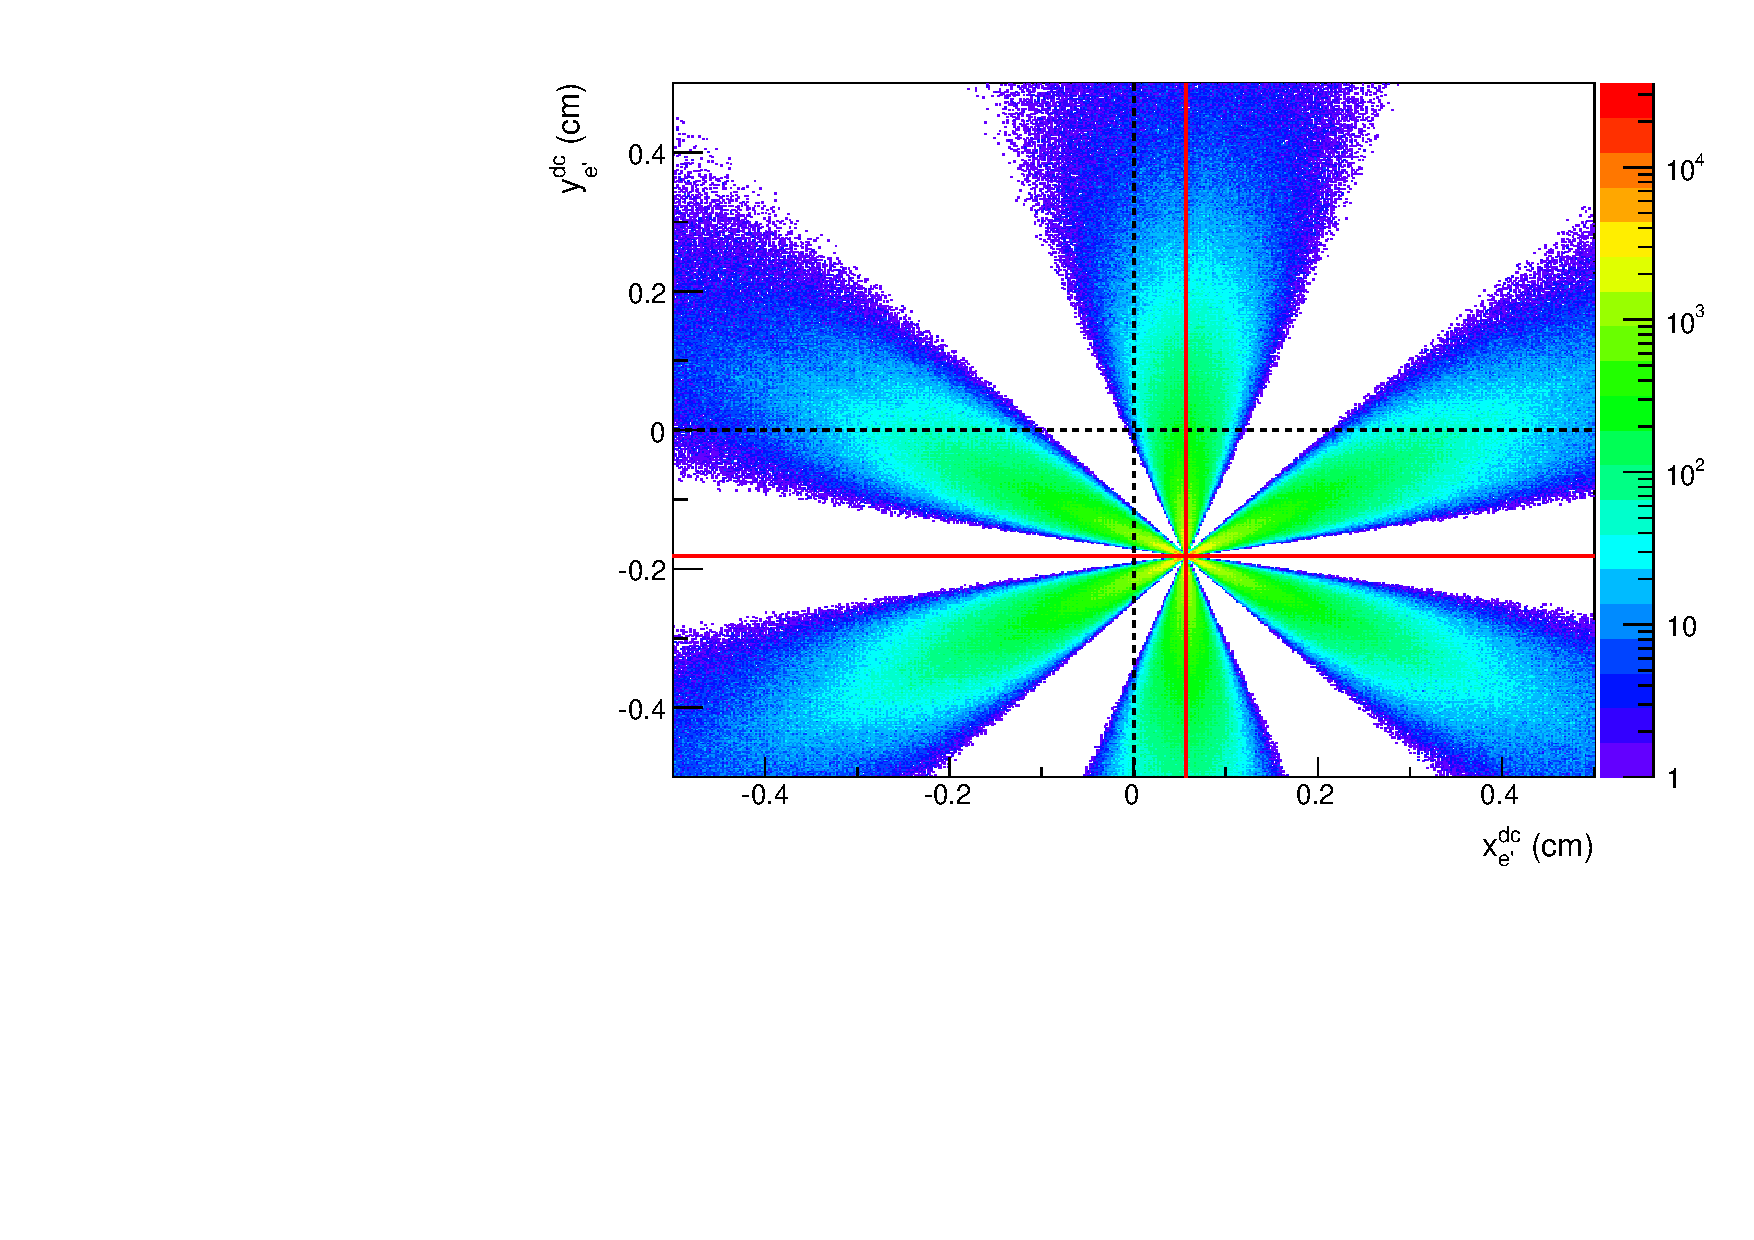
\includegraphics[width=11cm]{pictures/other_cuts/z_vertex/beam_offset.pdf}}
\end{center}
\caption{\small $y_{e'}^{dc}$ versus $x_{e'}^{dc}$ distribution that demonstrates the beam offset. Black dashed lines mark the position ($x$,~$y$) = (0,~0), where the beam is expected to be. Red lines demonstrate the actual beam position at ($x$,~$y$) = (0.057~cm,~-0.182~cm). }
\label{fig:beam_offset}
\end{figure}


In Fig.~\ref{fig:z_el_data_sim} event distributions after the subtraction of the empty target contribution are shown in comparison with Monte Carlo events reconstructed taking into account the beam offset. As can be seen in this figure the simulation matches the data well enough and almost completely reproduces the sector dependent deviation of the distributions from the nominal position marked by the black dashed lines.

To reduce the number of events in which the final state particles came from different events and/or took part in final state interactions, the following two additional cuts on the particle $z$-coordinates at the vertex are applied. The first cut is $|z_{h} + 0.4| < 4.4$~cm, where the index $h$ corresponds to the final hadron type (proton, $\pi^{+}$, and $\pi^{-}$). The left side of Fig.~\ref{fig:add_cuts_vert} shows an example of this cut for the case $h=\pi^{+}$. The second cut is $|z_{i} - z_{j}| < 5$~cm, where the indices $i$ and $j$ ($i\neq j$) correspond to the final particle type (electron, proton, $\pi^{+}$, and $\pi^{-}$). The right side of Fig.~\ref{fig:add_cuts_vert} shows an example of this cut for the case $i=\pi^{-},~j=\pi^{+}$. These additional cuts are made rather loose in order to avoid unjustified loss of good events.

\begin{figure}[!ht]
\begin{center}
\framebox{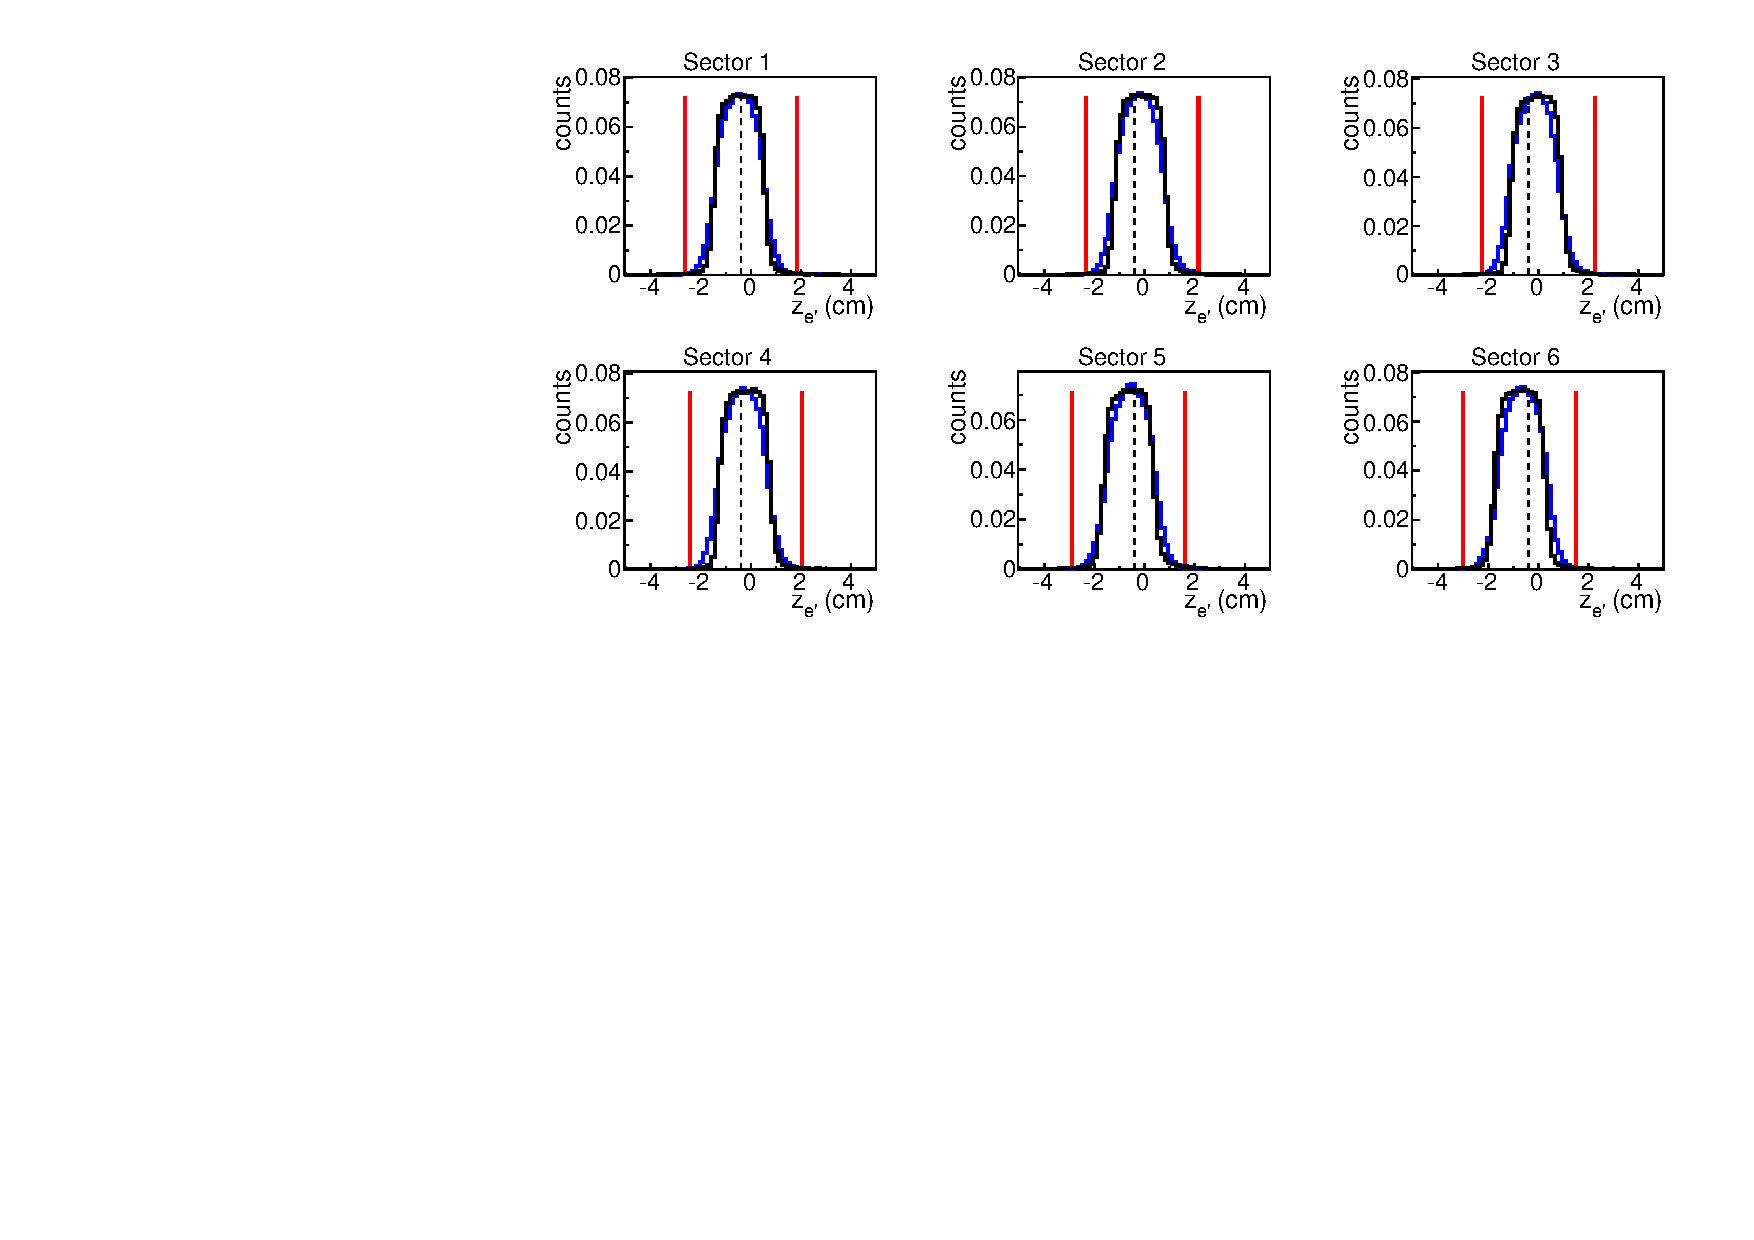
\includegraphics[width=13.1cm]{pictures/other_cuts/z_vertex/z_el_data_sim3.pdf}}
\end{center}
\caption{\small Distributions of the electron $z$-coordinate at the vertex for the experimental data (black curves) and the Monte Carlo events reconstructed taking into account the beam offset (blue curves) for the six CLAS sectors. For the data empty target contributions are subtracted. Vertical dashed lines mark the position $z = -0.4$~cm, where the center of the target is expected to be. Vertical red lines show the applied cuts. All distributions are normalized to the integral. }
\label{fig:z_el_data_sim}
\end{figure}

\begin{figure}[!ht]
\begin{center}
\framebox{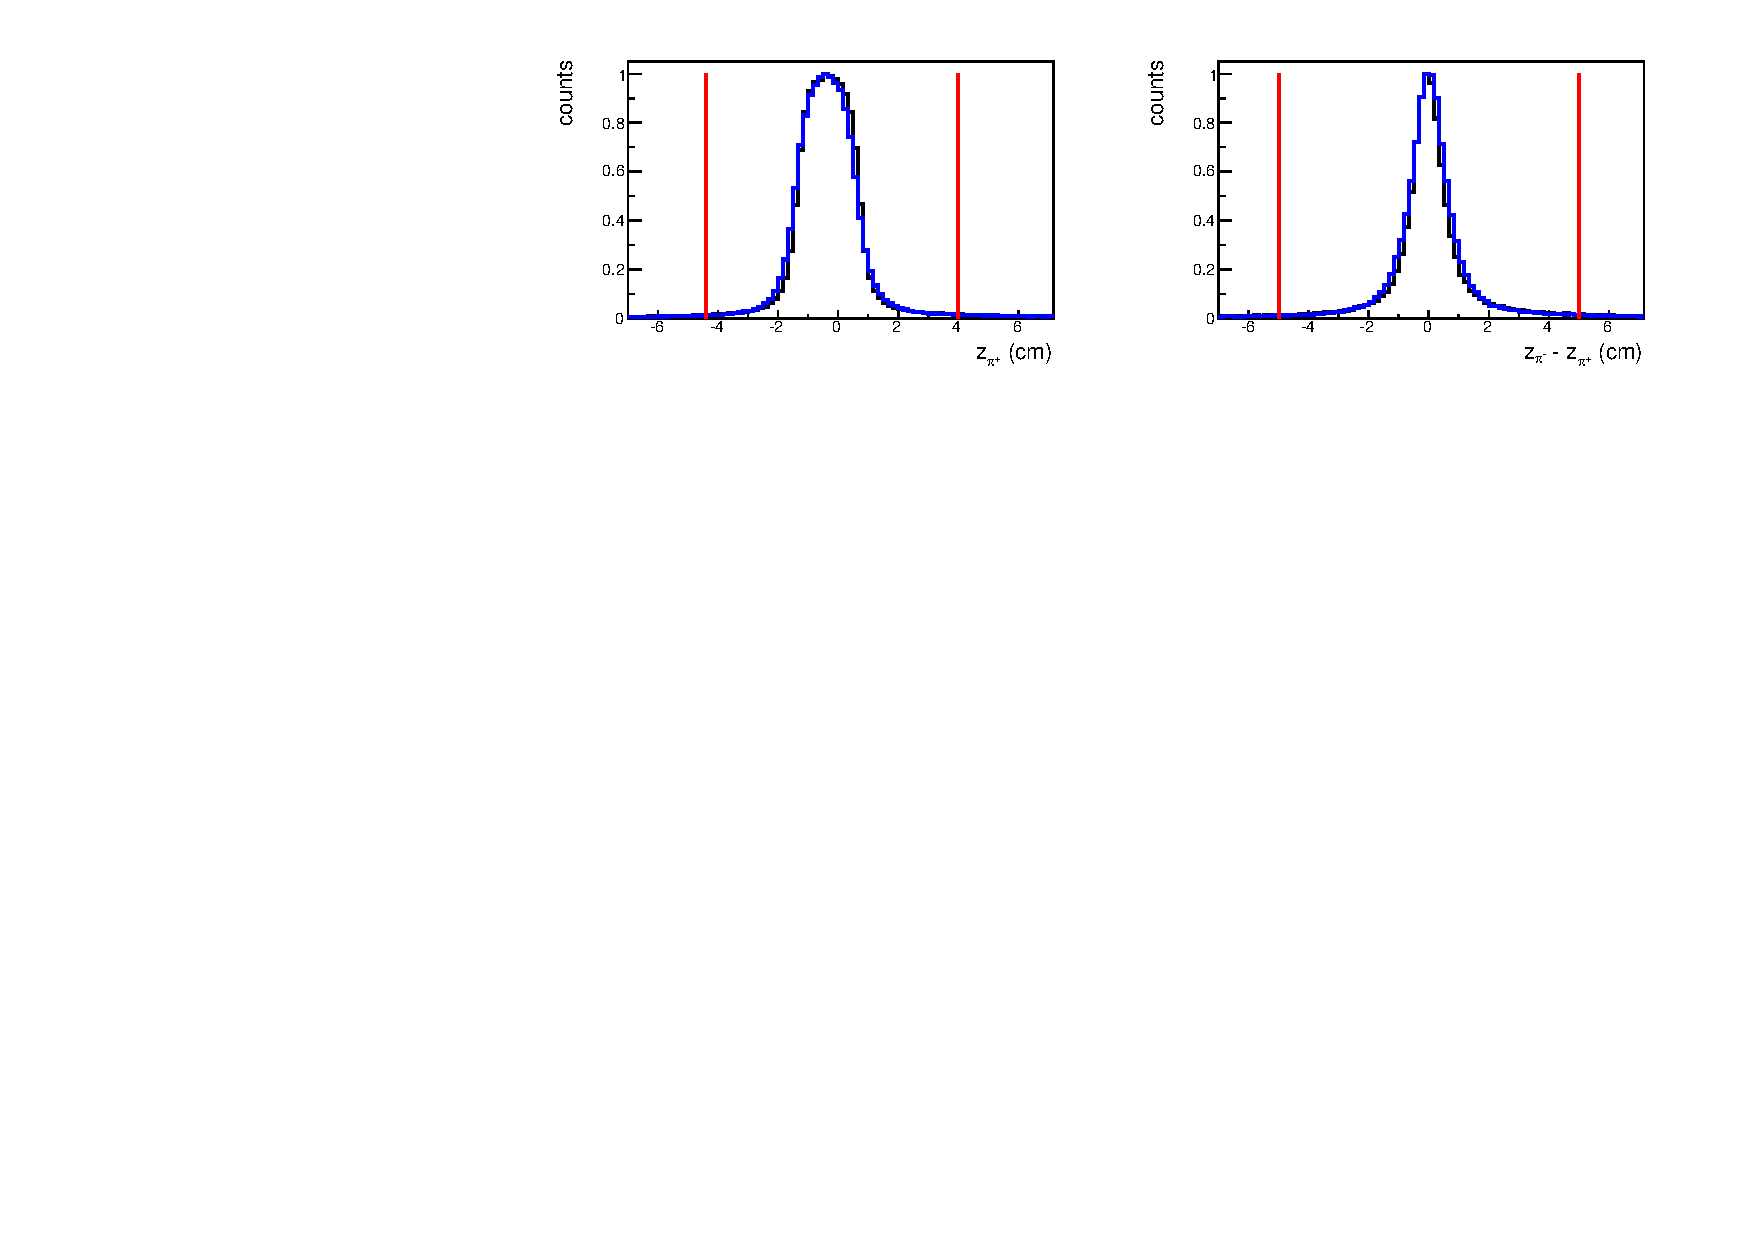
\includegraphics[width=13.1cm]{pictures/other_cuts/z_vertex/additional_cuts.pdf}}
\end{center}
\caption{\small Left plot: an example of the cut on the hadron $z$-coordinate, $|z_{\pi^{+}} + 0.4| < 4.4$~cm. Right plot: an example of the cut on the difference of the vertex $z$-coordinates of the final particles, $|z_{\pi^{-}} - z_{\pi^{+}}| < 5$~cm. The black curves correspond to the data, while the blue ones correspond to the reconstructed Monte Carlo events. All histograms are normalized to their maxima.}
\label{fig:add_cuts_vert}
\end{figure}



\newpage
\section{Exclusivity cut in the presence of Fermi smearing and FSI}
\label{Sect:excl_cut}

For picking out certain exclusive reactions one needs to register the scattered electron and either all final hadrons or all except one. In the latter case the four-momentum of the unregistered hadron can be restored using energy-momentum conservation (a so-called ``missing mass technique"). Thus for the reaction $e p \rightarrow e' p' \pi^{+} \pi^{-} $ one can in general distinguish between four so-called ``topologies" depending on the specific combination of registered final hadrons. In this particular analysis the following two topologies are analyzed,%\vspace{-0.25em}
\begin{itemize}
\item the fully exclusive topology (all final particles registered) $e p \rightarrow e' p' \pi^{+} \pi^{-} X$, and%\vspace{-0.25em}
\item the $\pi^{-}$ missing topology $e p \rightarrow e' p' \pi^{+} X$.
\end{itemize} %\vspace{-0.25em}


Due to the experimental conditions the statistics of the fully exclusive topology is very limited. This happens mainly because CLAS does not cover the polar angle range $0\,^{\circ}\mathrm{} < \theta_{lab} < 8\,^{\circ}\mathrm{}$~\cite{Mecking:2003zu}. The presence of this forward acceptance
hole does not affect much the registration of the positive particles ($p$ and $\pi^{+}$), since their trajectories are bent by the magnetic field away from the hole. Meanwhile, the negative particles ($e$ and $\pi^{-}$) are inbending, which means that their trajectories are bent into the forward direction. Electrons being very light and rapid undergo small track curvature, and the presence of the forward hole leads for them only to a constraint on the minimum achievable $Q^2$. However, for negative pions the situation is dramatic: being heavier and slower they are bent dominantly into the forward detector hole and, therefore, most of them cannot be registered. This leads to the fact that the $\pi^{-}$ missing topology contains the dominant part of the statistics. The contribution of the fully exclusive topology to the total analyzed statistics\footnote[7]{The combined statistics of both the $\pi^{-}$ missing and the fully exclusive topologies.} varies from $\sim$5\% near the reaction threshold to $\sim$25\% at $W\sim 1.7-1.8$~GeV. 
 
For reactions with multi-particle final states the problem of limited acceptance is an essential issue. Specifically, in the case of the $p\pi^{+}\pi^{-}$ final state the cross section  depends on five final hadron variables and hence is multi-dimensional, but the limited statistics only allows the extraction of a set of one-fold differential cross sections (see Sects.~\ref{Sect:kin_var} and ~\ref{Sect:cr_sect_formula}). This leads to the necessity to fill kinematic cells with zero acceptance (so-called ``empty cells") based on some model assumptions, which leads to model dependent results (see Sect.~\ref{Sect:empt_cells}). The fully exclusive topology suffers from the problem of limited acceptance (and therefore large amount of empty cells) that along with the problem of limited statistics does not allow any sensible cross section information to be obtained from this topology alone. The $\pi^{-}$ missing topology, having significantly fewer empty cells, serves the purpose of the cross section extraction best. The use of both topologies combined allows the model dependence of the cross section (that originates from empty cells filling) to be reduced as well as slightly increasing the statistics.

The aforementioned features of the two topologies are caused by the experimental conditions and valid either for an experiment off the free proton or for one off the proton bound in the deuteron. Meanwhile, there are also some features that appear only in bound proton experiments. Those that are crucial for exclusive event selection are addressed later in this Section, while others are discussed later in the report.% they are mentioned later in this Section and discussed in Sect.~\ref{Sect:?}.

Actually, two more topologies can be distinguished, i.e. the proton missing topology and the $\pi^{+}$ missing topology. Both require registration of the $\pi^{-}$ in the final state and as a consequence suffer from the similar problems of suppressed statistics\footnote[8]{Each of them contains about 10\% of the full statistics of all four topologies combined.} and limited acceptance as in the case of the fully exclusive topology.  Therefore, these two topologies are usually ignored in analyses of the reaction $ep\rightarrow{}e'p'\pi^{+}\pi^{-}$~\cite{Rip_an_note:2002,Ripani:2002ss,Fed_an_note:2007,Fedotov:2008aa,Isupov:2017lnd}. Nevertheless, as demonstrated in the sophisticated analysis of this reaction off the free proton target~\cite{Fed_an_note:2017,Fed_paper_2018}, they can be used as complimentary topologies to the main $\pi^{-}$ missing topology, that allows a slight increase in the statistics and a reduction in the amount of empty cells as much as possible, therefore minimizing the model dependence of the extracted cross sections. However, if the pion pair is produced off the proton bound in the deuteron, additional complications appear: these topologies turn out to be polluted with events from other reaction channels. In the proton missing topology the missing mass technique fails to distinguish whether the pion pair was produced off the proton or off the neutron, because their masses are almost identical. A similar situation occurs for the $\pi^+$ missing topology, where the same reason prevents distinguishing between the production of $\pi^{+}\pi^{-}$ pair off the proton and $\pi^{0}\pi^{-}$ pair off the neutron, if only the proton and the $\pi^{-}$ in the final state are registered. Moreover, the event sample in the $\pi^+$ missing topology demonstrates strong admixture of events from the reaction $en(p)\rightarrow e'p'(p')\pi^{-}$, which was found to be not very easy to remove.
 
Taking into account all the above arguments, the following topology ranking takes place in this particular analysis: the $\pi^{-}$ topology is the main one and the fully exclusive topology is treated as the complimentary one, which gives a slight increase in statistics as well as some reduction in the amount of empty cells, while the proton missing and the $\pi^{+}$ missing topologies are not used at all.

Meanwhile, an exclusive reaction that happens off bound nucleons has some specific features, which are extrinsic to reactions off free protons. Those of them that are related to the problem of the channel identification are listed below.%\vspace{-0.25em}

\begin{itemize}
\item  The Fermi motion of the target proton.% \vspace{-0.25em}
\item Complex effects of Final State Interactions (FSI) due to the presence of the neutron and the multi-particle final state.
\end{itemize}%\vspace{-0.25em}

\everypar{\looseness=-1}
The manifestations of these effects in the $\pi^{-}$ missing and fully exclusive topologies differ.

Motion of the target proton within the deuterium nucleus is concealed from the observer and is not measured\footnote[9]{In general it can be measured by detecting the recoil nucleon (neutron in this case), but it was not an option in this experiment.}. However, if all particles in the final state are registered, one can restore the information about the momentum distribution of the target proton via energy-momentum conservation (see Sect.~\ref{Sect:excl_cut_fully_excl} for details). This is not the case for the $\pi^{-}$ missing topology, where incomplete knowledge about the final state leads to the fact that information about the motion of the initial proton turns out to be totally lost. Therefore, one is forced to work under a so-called ``target-at-rest-assumption" that considers the target proton to have no motion and as a consequence inevitably leads to the smearing of various kinematic quantities, such as missing mass, reaction invariant mass ($W$), etc~\cite{Skorodumina:2015rea}. 
Although the fully exclusive topology has the advantage of the possibility of avoiding the smearing\footnote[10]{For example, in the fully exclusive topology the value of $W$, being calculated using the four-momenta of the registered final hadrons, turns out to be determined within the detector resolution and not affected by the effects of the target motion.}, all kinematic quantities are nevertheless calculated under the target-at-rest-assumption in order to treat this complimentary topology in the same way as the main one.


In order to reliably identify the exclusive channel and correctly calculate the detector efficiency, the distributions of the reconstructed Monte Carlo events must match experimental ones as well as possible. As mentioned above, the necessity to work under the target-at-rest-assumption smears the experimental distributions, which in turn demands the simulated distributions reproduce this smearing. Therefore, the effects of the target motion should be properly included in the Monte Carlo simulation.

\everypar{\looseness=-1}
That is why the event generator TWOPEG-D~\cite{twopeg-d} was used to perform the Monte Carlo simulation. It is a version of the TWOPEG (event generator for double-pion electroproduction off the free proton~\cite{twopeg}) that was developed for this analysis in order to simulate the effects of the target motion. In this version of the event generator the Fermi motion of the initial proton is generated according to the Bonn potential~\cite{Machleidt:1987hj} and then naturally merged into the specific kinematics of double-pion electroproduction.


The second intrinsic feature of an exclusive reaction off bound nucleons is complex effects of FSI. This phenomenon is driven by the strong interaction and consists in the fact that after the production of the final state hadrons and before their registration they manage to interact with each other and/or the recoil nucleon. 

Final hadrons produced off free protons are subject to FSI as well, but they are limited to interactions of the hadrons with each other, which are not substantial. Meanwhile, for reactions off protons in deuterium, the presence of spectator neutrons changes the situation drastically as the final hadrons can impact the neutron. As a result, FSI effects in such reactions are rather strong. 


Events, in which all final hadrons manage to avoid FSI, belong to a so-called ``quasi-free regime". Meanwhile, events with FSI-affected hadrons are attributed to so-called ``FSI-disturbed kinematics" because FSI alter the final hadron momenta. Events in FSI-disturbed kinematics introduce distortions into distributions of various kinematic quantities, such as missing masses, thus complicating the identification of a desired exclusive channel.


The main goal of this study is to extract the double-pion cross sections in the quasi-free regime, which implies the need to select for the analysis only events in quasi-free kinematics and to get rid of events with FSI. The latter, however, also deserve attention as FSI effects represent an essential issue in studies of any exclusive reaction, especially off nuclei. Therefore, to balance the analysis, Chapter~\ref{Sect:fsi_discuss} of the thesis is fully devoted to the examination of features and manifestations of FSI-affected events.


\everypar{\looseness=-1}
In contrast to the effects of the target motion, which can be simulated fairly easy, the effects of FSI can hardly be taken into account in the simulation because they are of very complex nature and hence not yet fully understood. Therefore, the Monte Carlo simulation is not able to reproduce the distortions due to FSI that occur in some experimental distributions, but this is not a problem if events in quasi-free kinematics are properly separated from those in FSI-disturbed kinematics. This leads to the necessity to develop special procedures of selecting quasi-free events as well as correcting for the remaining admixture of undesired events, if they cannot be fully eliminated.


The yield of events in FSI-disturbed kinematics turned out to strongly depend on (i) the reaction invariant mass ($W$) and (ii) on the hadron scattering angles. The latter issue causes FSI effects to manifest themselves differently depending on the reaction topology, since the topologies have non-identical geometrical acceptance.%, that in turns forces us to select quasi-free event in each topology individually. 

As follows from the above, the two analyzed topologies differ from each other both in treating of the Fermi motion of the initial proton and in FSI manifestations. Therefore, the channel identification is performed in each topology individually (see subsequent subsections). 


The problem of background channels is also an issue that deserves special attention. For the reaction of double-pion production off free protons, the main background channel is $ep\rightarrow e'p'\pi^{+}\pi^{-}\pi^{0}$. In the analysis~\cite{Fed_an_note:2017} that was carried out for the same beam energy $E_{beam} = 2.039$~GeV, it is shown that although the admixture of the events from this background channel becomes discernible at $W\gtrsim 1.6$~GeV, it remains negligible and well separated from the double-pion events via the exclusivity cuts. For the experiments with the deuteron target, the reaction $en(p) \rightarrow e'p'(p')\pi^{+}\pi^{-}\pi^{-}$ can also act as a background channel for the investigated $ep(n) \rightarrow e'p'(n')\pi^{+}\pi^{-}$ reaction, however it is also expected to give an insignificant and well separated admixture. Here and hereinafter the term ``background channel" is used to denote the reaction that happened in electron scattering off the target nucleon along with the investigated double-pion reaction. Any reaction that might occur during the FSI is not treated as the contribution from ``background channels", but is attributed to the FSI-background.



\subsection{Fully exclusive topology}
\label{Sect:excl_cut_fully_excl}


In the fully exclusive topology for the selection of double-pion events in quasi-free kinematics the distributions of the following quantities were investigated: the missing momentum $P_{X}$ and the missing mass squared $M^{2}_{X[0]}$ for the reaction $ep(n)\rightarrow e'p'(n')\pi^{+}\pi^{-}X$ as well as the missing mass squared $M^{2}_{X[\pi^{-}]}$ for the reaction $ep(n)\rightarrow e'p'(n')\pi^{+}X$. These quantities are defined by\vspace{-1em}
\begin{equation}
\begin{aligned}
&P_{X}&=&~|\overrightarrow{P}_{e} - \overrightarrow{P}_{e'}- \overrightarrow{P}_{p'} - \overrightarrow{P}_{\pi^{+}} - \overrightarrow{P}_{\pi^{-}}|,\\[-2pt]
&M_{X[0]}^{2}&=&~[P_{e}^{\mu} + P_{p}^{\mu}- P_{e'}^{\mu}- P_{p'}^{\mu}-  P_{\pi^{+}}^{\mu} - P_{\pi^{-}}^{\mu}]^{2},\\[-2pt]
&M_{X[\pi^{-}]}^{2}&=&~[P_{\pi^{-}~miss}^{\mu}]^{2}=[P_{e}^{\mu} + P_{p}^{\mu}- P_{e'}^{\mu}- P_{p'}^{\mu}-  P_{\pi^{+}}^{\mu}]^{2},\\[-12pt]
\end{aligned}\label{eq:excl_top_quant}
\end{equation}%\vspace{-0.5em}
where $P_{i}^{\mu}$ are the four-momenta and $\overrightarrow{P_{i}}$ the three-momenta of the particle $i$. All three quantities are calculated under the target-at-rest-assumption, i.e. considering $P^{\mu}_{p} = (0,~0,~0,~m_{p})$, where $m_{p}$ is the proton mass.


\afterpage{\clearpage}
%\clearpage
\begin{figure}[!ht]
\begin{center}
\framebox{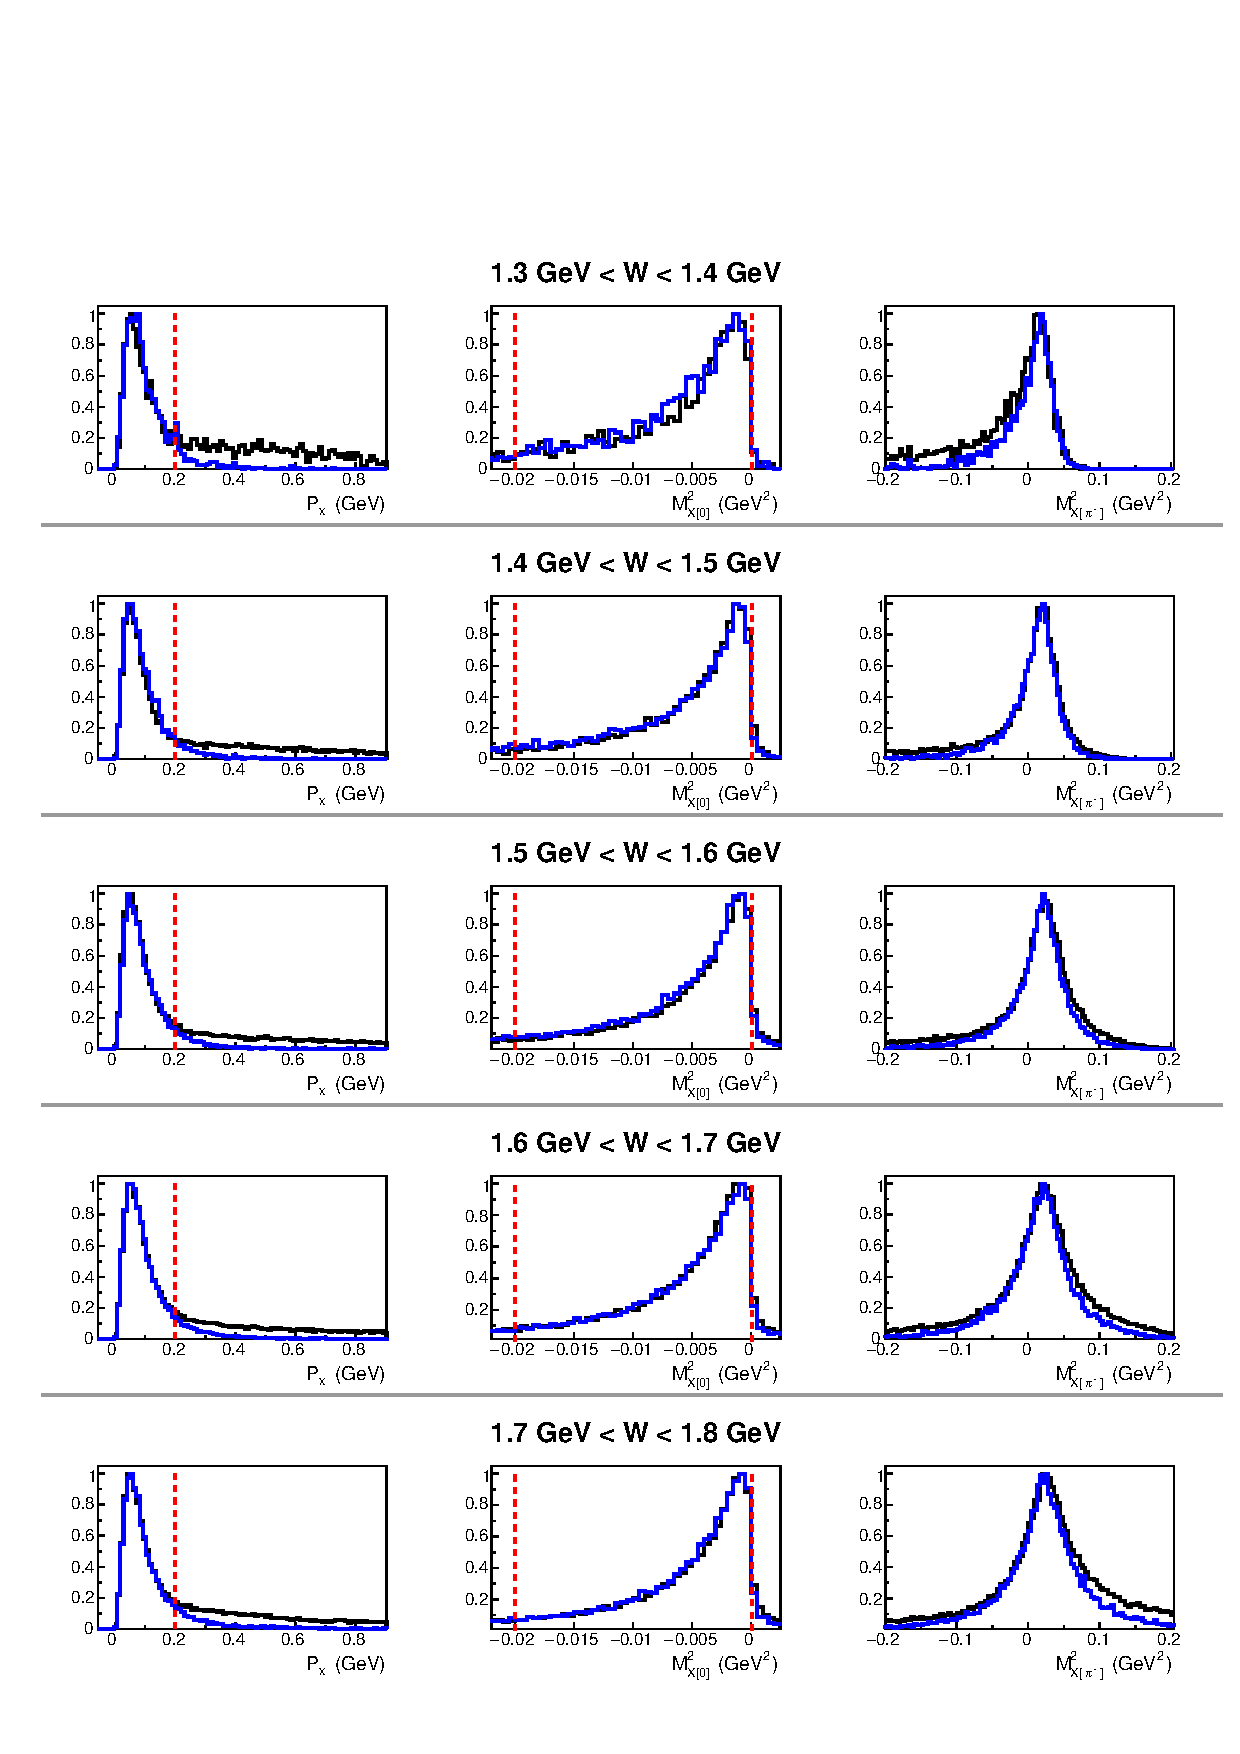
\includegraphics[width=\textwidth]{pictures/other_cuts/excl_cut/excl_top.pdf}}
\end{center}
\caption{\small Distributions of the quantities $P_{X}$ (left column), $M^{2}_{X[0]}$ (middle column), and $M^{2}_{X[\pi^{-}]}$ (right column) defined in Eq.~\eqref{eq:excl_top_quant} for experimental data (black curves) and Monte Carlo simulation (blue curves) for different 100-MeV-wide $W$ bins. Vertical red lines indicate the cuts applied for the selection of exclusive quasi-free events. All plotted quantities as well as the values of $W$ are calculated under the target-at-rest-assumption. All distributions are normalized to their maxima.}
\label{fig:excl_top}
\end{figure}



The quantities $P_{X}$ and $M^{2}_{X[0]}$ are unique for the fully exclusive topology as they can be calculated only if all final hadrons are registered. Although adding the quantity $M_{X[\pi^{-}]}^{2}$ to this set does not seem to provide any additional information, it is examined in order to observe consistency with the $\pi^{-}$ missing topology, where the distributions of $M_{X[\pi^{-}]}^{2}$ is the only source for developing a criterion for the channel identification. See Ref.~\cite{note_mm_distr} for details on features of missing mass distributions.

\everypar{\looseness=-1}
Distributions of the quantities $P_{X}$ (first column), $M^{2}_{X[0]}$ (second column), and $M_{X[\pi^{-}]}^{2}$ (third column) for five 100-MeV-wide bins\footnote[11]{The value of $W$ is calculated for the initial state under the target-at-rest-assumption.} in $W$ are shown in Fig.~\ref{fig:excl_top} for the experimental data (black curves) and reconstructed Monte Carlo events (blue curves).

%by $W = \sqrt{(P_{e}^{\mu} + P_{p}^{\mu}- P_{e'}^{\mu})^{2}}$.

The quantity $P_{X}$ (first column in Fig.~\ref{fig:excl_top}) is the missing momentum of the initial proton calculated under the target-at-rest-assumption, therefore the blue curves stand for the Fermi momentum (simulated according to Bonn potential~\cite{Machleidt:1987hj}) convoluted with the detector resolution, whereas the black ones correspond to the experimental momentum of the initial proton, mixed with the FSI effects, contributions from background channels, and the detector resolution. As seen in the left column of Fig.~\ref{fig:excl_top}, the simulated distributions perfectly match the experimental ones for $P_{x} < 0.2$~GeV, while for $P_{x} > 0.2$~GeV the simulation underestimates data. Such behavior is mostly related to the fact that relative contributions from FSI, which were not included into the Monte Carlo simulation, turn out to be the most significant outside of the peak region. The background channels, being not included into the Monte Carlo as well, also contribute to this mismatch, but as mentioned above their contribution is minor.
The value  $P_{x} = 0.2$~GeV (marked by the red dashed lines in each plot in the left column) was chosen as a criterion for the selection of events in quasi-free kinematics. Thus, experimental events located at the left side of this line correspond to the reaction in the quasi-free regime, while events at the right side correspond mostly to ``disturbed" kinematics with great impact of FSI.

The distributions of the quantity $M^{2}_{X[0]}$ shown in the middle column in Fig.~\ref{fig:excl_top} deserve more attention. As demonstrated in Refs.~\cite{Fed_an_note:2017,Fed_paper_2018,note_mm_distr}, in free proton experiments this quantity forms a very narrow peak at zero position barely affected either by radiative effects or by detector resolution. An admixture from the three-pion background, if present in the analyzed event sample, forms then an additional peaked structure at $m_{\pi}^{2}$ well-separated from the main distribution peak. Meanwhile, in this analysis, $M^{2}_{X[0]}$, being calculated under the target-at-rest-assumption, loses its thinness and acquires the smearing (mostly left-sided), which is well-reproduced by the Monte Carlo simulation.

In order to clean up the sample of exclusive events, the cut on the missing mass squared $M^{2}_{X[0]}$ was also applied as a complementary to the cut on the missing momentum. This cut is shown in Fig.~\ref{fig:excl_top} (middle column) by the vertical red dashed lines. The plots in the middle column are zoomed near the peak to demonstrate good agreement between the data and the simulation within the cut limits. The behavior of $M^{2}_{X[0]}$ in a wider range is shown in Fig.~\ref{fig:mm_0_zoomed}, where the distributions are zoomed in on small $y$. As seen, outside the cut boundaries there is a mismatch between the data and simulation, which originates from FSI effects at the left and the contribution from the three-pion background at the right. The latter forms a peaked structure around $m_{\pi}^{2}$ ($\sim$0.02~GeV$^{2}$), which is more smeared compared to the free proton case due to the target-at-rest-assumption and FSI disturbances. The example is given for high $W$ to observe the greatest background admixture over the investigated $W$ range.

\begin{figure}[!ht]
\begin{center}
\framebox{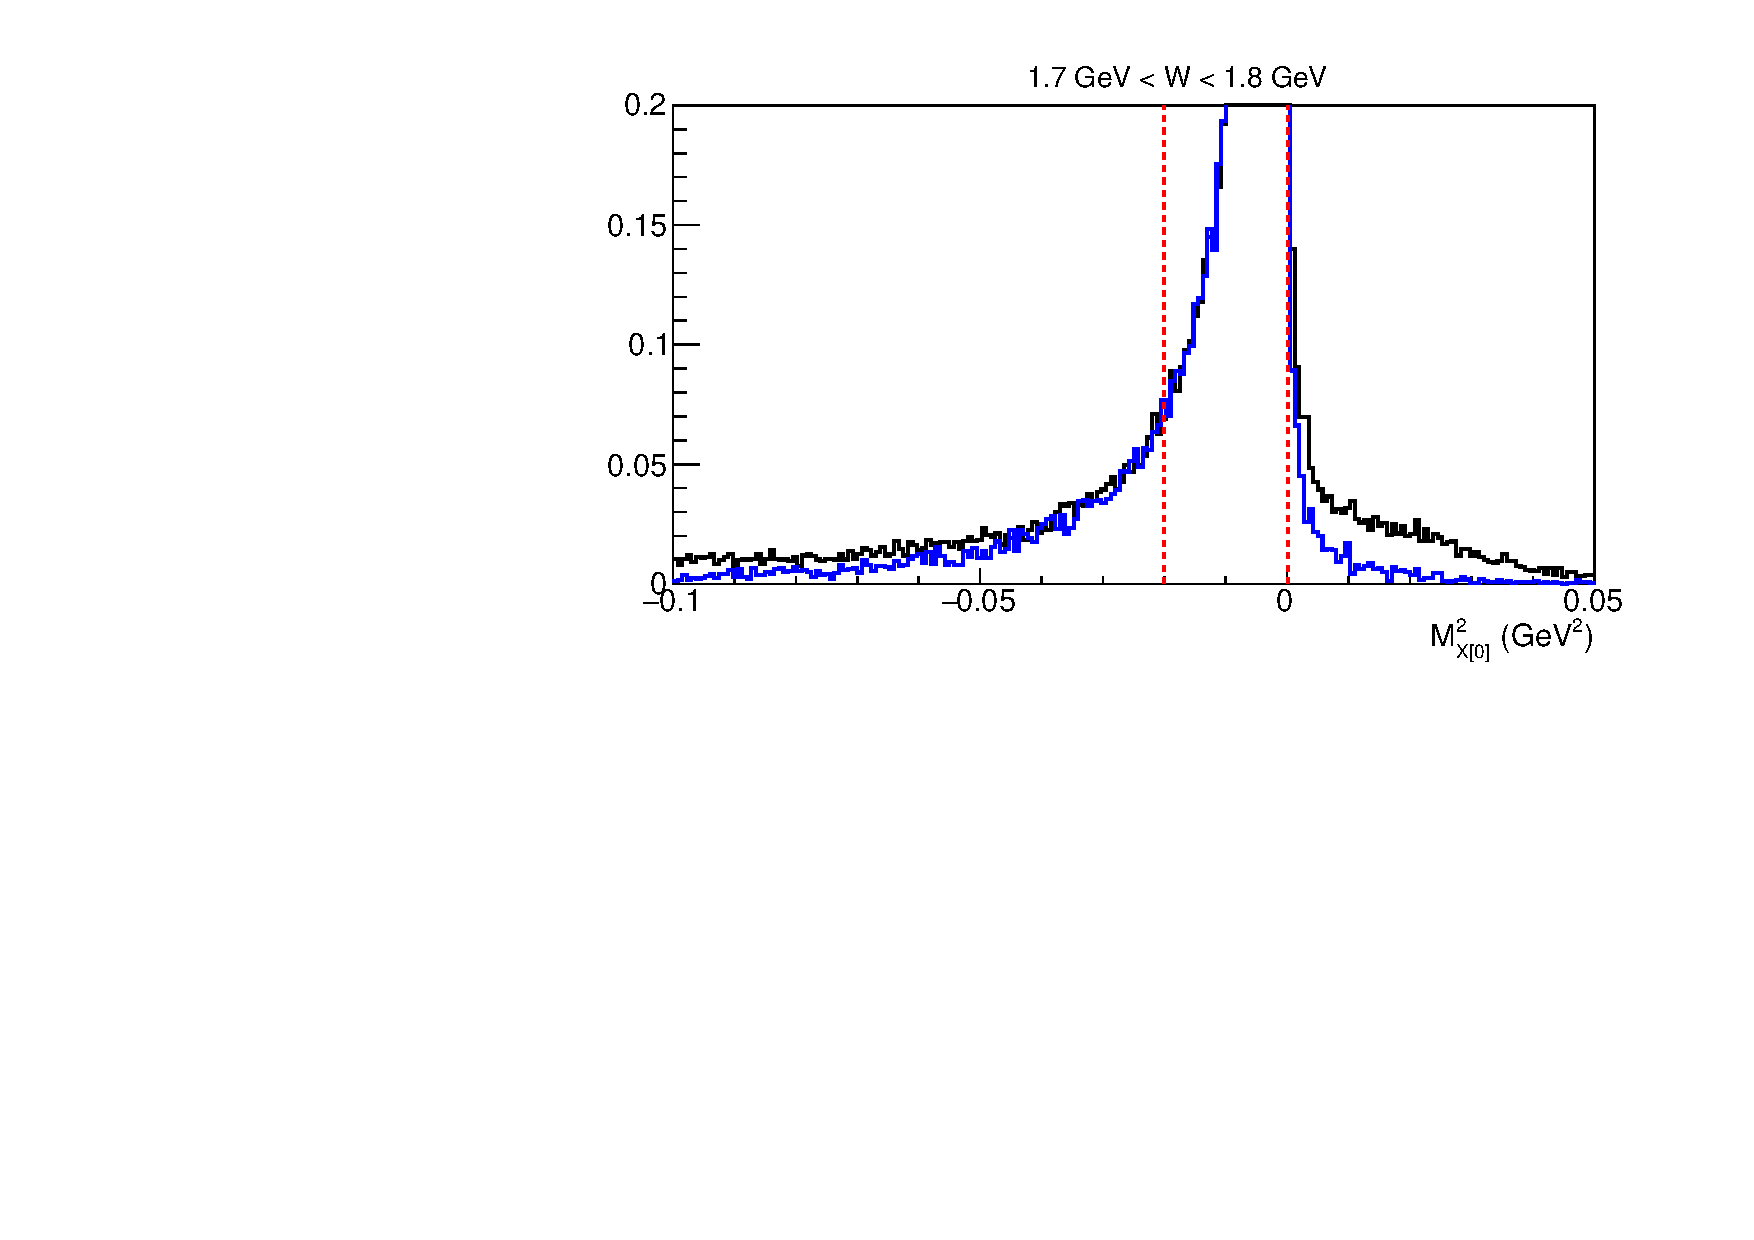
\includegraphics[width=13.1cm]{pictures/other_cuts/excl_cut/mm_0_zoomed.pdf}}
\end{center}
\caption{\small Distributions of the quantity $M^{2}_{X[0]}$ for experimental data (black curves) and Monte Carlo simulation (blue curves) zoomed in on small $y$. Vertical red lines indicate the applied cut. The mismatch between data and simulation originates from FSI effects at the left and three-pion background at the right. The example is given for 1.7~GeV $< W <$ 1.8~GeV, where the latter is greatest over the whole $W$ range. The agreement between data and simulation within the cut boundaries is better shown in Fig.~\ref{fig:excl_top} (middle column).}
\label{fig:mm_0_zoomed}
\end{figure}



The three-pion background in this topology is thus considered to be fully eliminated by the described above cuts on the quantities $P_{X}$ and $M^{2}_{X[0]}$.


Meanwhile, the right column in Fig.~\ref{fig:excl_top} stands for the missing mass squared $M_{X[\pi^{-}]}^{2}$ defined by Eq.~\eqref{eq:excl_top_quant} under the target-at-rest-assumption, thus being Fermi smeared. The observed mismatch between the measured and simulated distributions is $W$-dependent and caused mostly by the FSI effects. 
\begin{figure}[!ht]
\begin{center}
\framebox{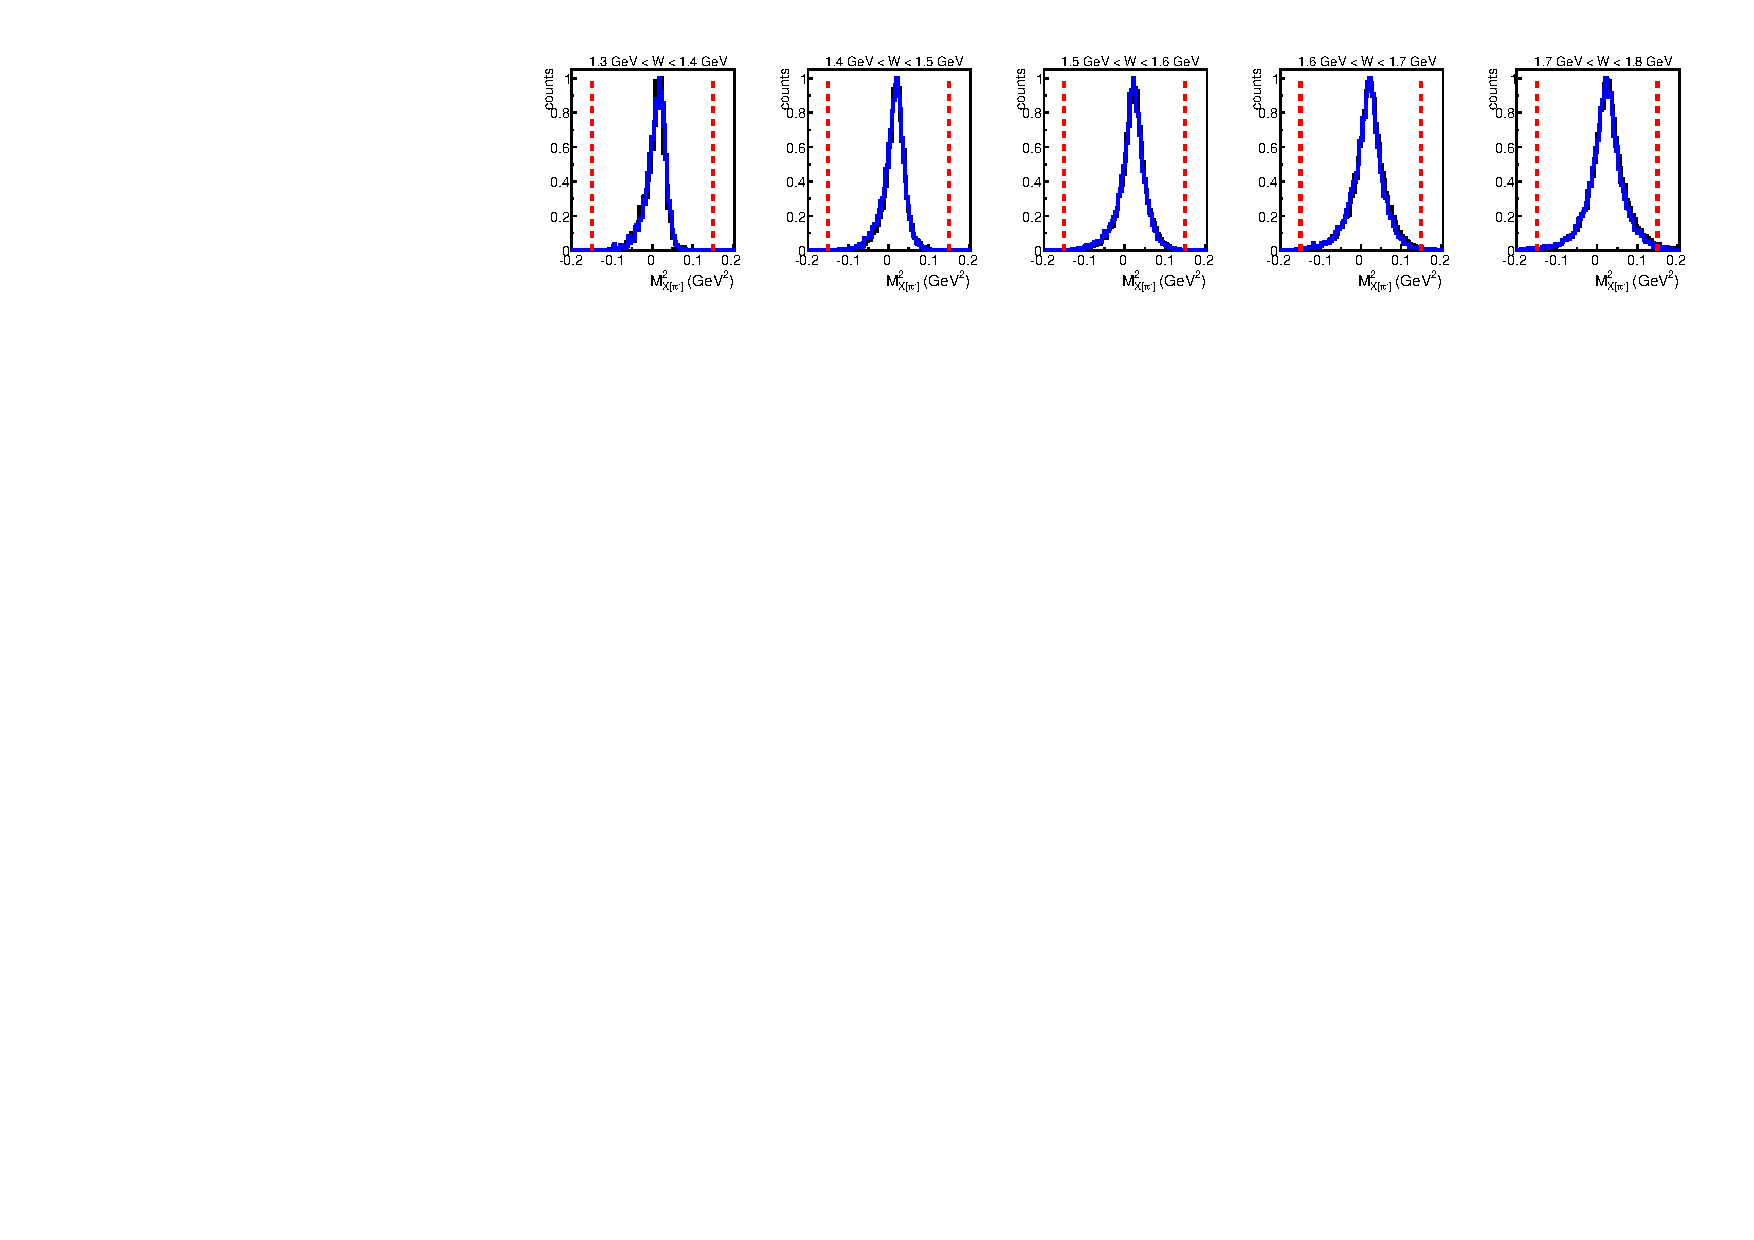
\includegraphics[width=\textwidth]{pictures/other_cuts/excl_cut/excl_top_aft_cut.pdf}}
\end{center}
\caption{\small Distributions of the missing mass squared $M^{2}_{X[\pi^{-}]}$ defined in Eq.~\eqref{eq:excl_top_quant} for the fully exclusive topology plotted for selected quasi-free exclusive events for experimental data (black curves) and Monte Carlo simulation (blue curves). The comparison is shown for different 100-MeV-wide $W$ bins. The quantity $M^{2}_{X[\pi^{-}]}$ as well as the values of $W$ are calculated under the target-at-rest-assumption. The vertical red lines show the applied cuts. All distributions are normalized to their maxima. See text for details. }
\label{fig:excl_top_aft}
\end{figure}

Figure~\ref{fig:excl_top_aft} shows the distributions of the quantity $M_{X[\pi^{-}]}^{2}$ plotted for quasi-free exclusive events selected by the cuts on $P_{x}$ and $M^{2}_{X[0]}$. The distributions for the experimental (black curves) and reconstructed Monte Carlo (blue curves) events perfectly match each other in all $W$ subranges, which demonstrates the reliability of quasi-free exclusive event selection as well as the fact that effects of the target motion are correctly implemented into the simulation. The vertical red lines in Fig.~\ref{fig:excl_top_aft} correspond to the additional cut that was applied on the missing mass squared $M_{X[\pi^{-}]}^{2}$.

Although in the fully exclusive topology the four-momentum of the $\pi^{-}$ is measured precisely within the detector resolution, it is not used in the subsequent calculation of kinematic variables for the cross section extraction. The measured four-momentum is instead replaced by the one that is calculated as missing ($P_{\pi^{-}~miss}^{\mu}$ in Eq.~\eqref{eq:excl_top_quant}) and thus is Fermi smeared. This is done to imitate the event selection in the main $\pi^{-}$ missing topology in order to treat events in both topologies identically. 

\newpage
\subsection{$\pi^{-}$ missing topology}
\label{Sect:excl_cut_pim_miss}

In the $\pi^{-}$ missing topology the quantities $P_{X}$ and $M^{2}_{X[0]}$ defined in Eq.~\eqref{eq:excl_top_quant} are not available due to the incomplete knowledge about the final state, and $M_{X[\pi^{-}]}^{2}$ is the only remaining quantity suitable for the selection of exclusive events in quasi-free kinematics. The distributions of this quantity are shown in Fig.~\ref{fig:main_top_mm2} for five 100-MeV-wide bins in $W$ for the experimental data (black curves) and the Monte Carlo simulation (blue curves). The comparison shown in this figure demonstrates again the $W$-dependent mismatch between data and simulation, which is different from that seen in the fully exclusive topology. The mismatch is mostly observed at the right side of the distribution peak and becomes discernible only for $W\gtrsim 1.5$~GeV.
\begin{figure}[!ht]
\begin{center}
\framebox{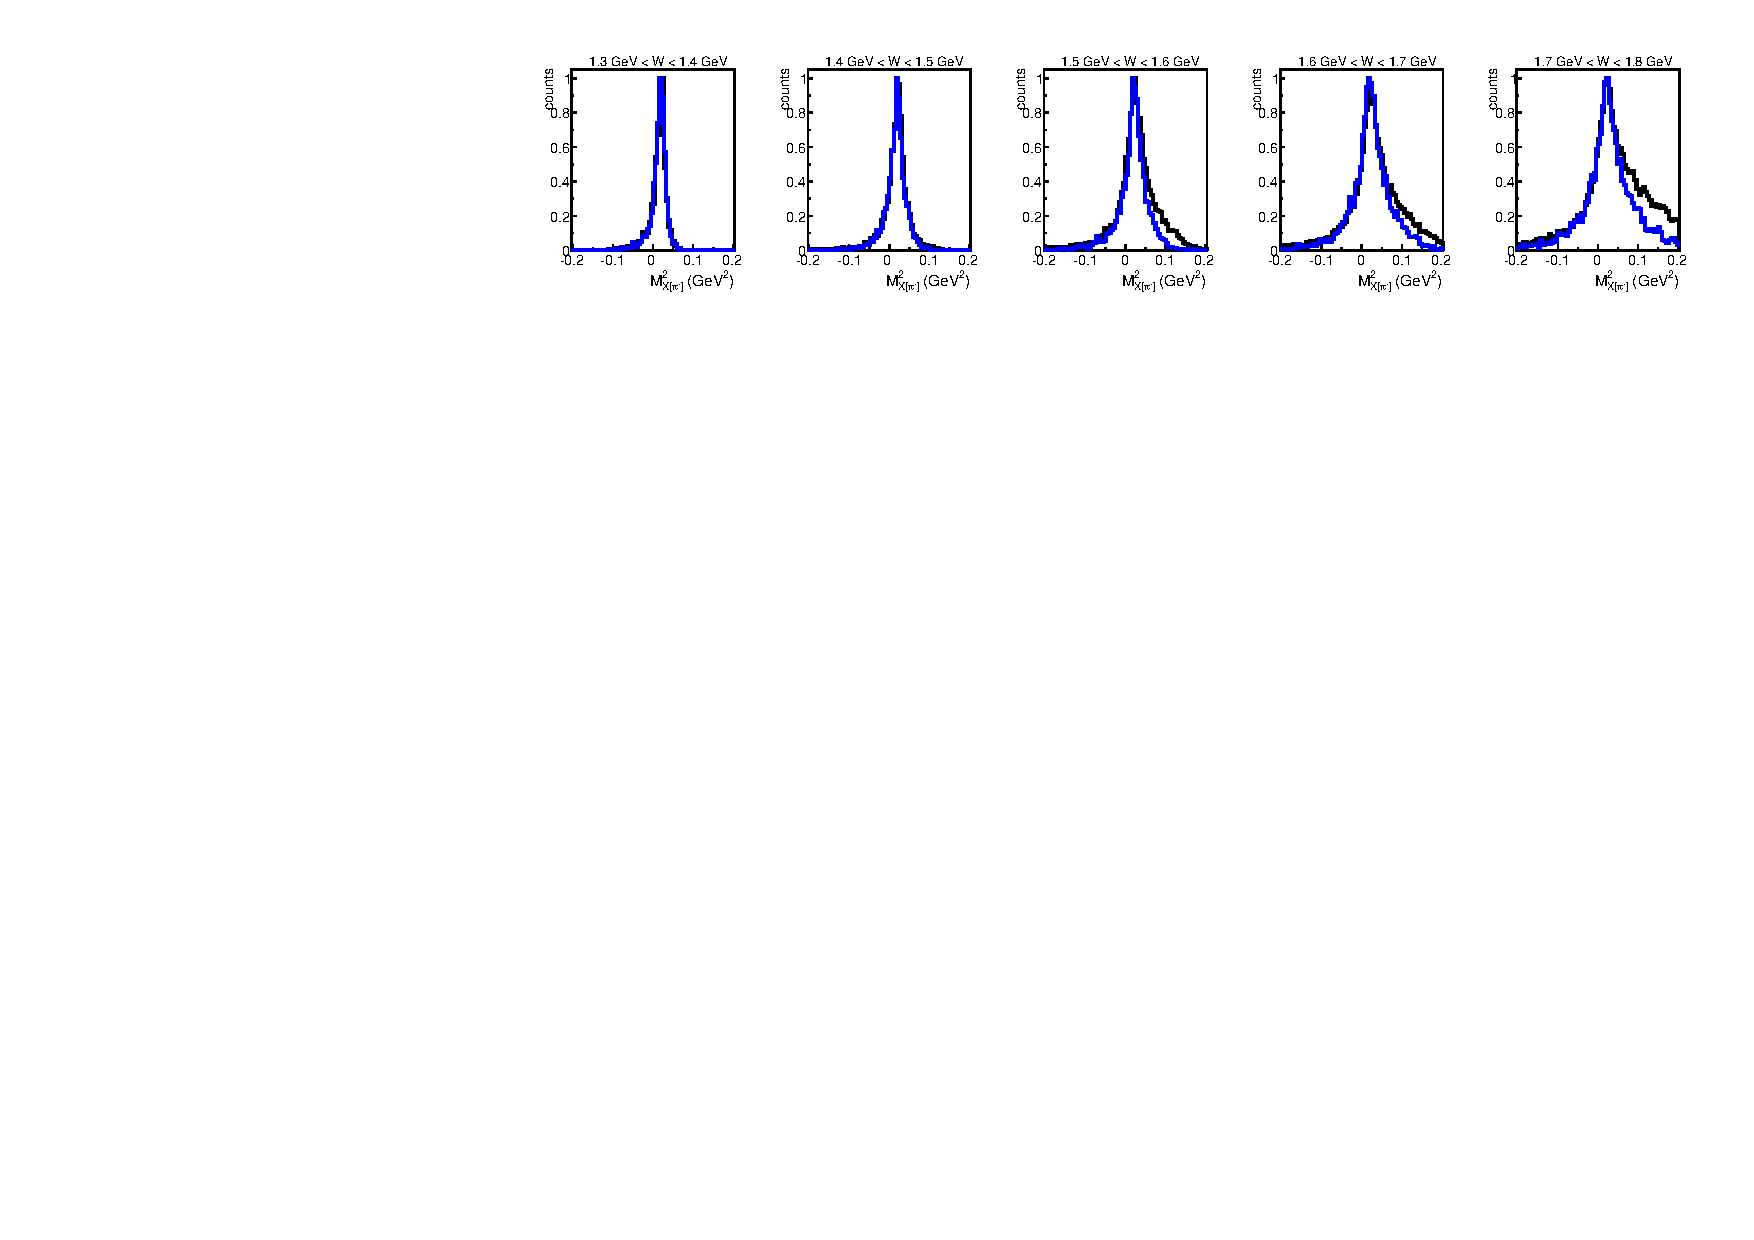
\includegraphics[width=\textwidth]{pictures/other_cuts/excl_cut/main_top_mm2.pdf}}
\end{center}
\caption{\small Distributions of the missing mass squared $M^{2}_{X[\pi^{-}]}$ defined in Eq.~\eqref{eq:excl_top_quant} for the $\pi^{-}$ missing topology plotted before the selection of quasi-free exclusive events for experimental data (black curves) and Monte Carlo simulation (blue curves). The comparison is shown for different 100-MeV-wide $W$ bins. The quantity $M^{2}_{X[\pi^{-}]}$ as well as the values of $W$ are calculated under the target-at-rest-assumption. All distributions are normalized to their maxima. See text for details. }
\label{fig:main_top_mm2}
\end{figure}

The similar analysis~\cite{Fed_an_note:2017} carried out for the same beam energy but off a free proton target did not reveal any substantial discrepancies between the experimental and simulated distributions of the quantity $M_{X[\pi^{-}]}^{2}$; they are shown to be in a very good agreement for all $W$ values. Figure~\ref{fig:excl_top_aft} plotted for selected exclusive quasi-free events in the fully exclusive topology in turn proves that the Monte Carlo simulation incorporates effects of the target motion correctly. Therefore, the discrepancy between data and simulation observed in Fig.~\ref{fig:main_top_mm2} is attributed mainly to the FSI effects, which are not included into the simulation.

This mismatch between data and simulation together with the fact that in the $\pi^{-}$ missing topology the quantity $M_{X[\pi^{-}]}^{2}$ is the only one available for the channel identification makes the task of selecting events in quasi-free kinematic rather challenging. To accomplish this goal, a special procedure was developed. This procedure is described below. 

\everypar{\looseness=-1}
In order to isolate events in quasi-free kinematics, the following quantity is subjected to examination,%\vspace{-1em}
\begin{equation}
 M_{X[\pi^{-}]}=\sqrt{|M_{X[\pi^{-}]}^{2}|}=\sqrt{|[P_{\pi^{-}~miss}^{\mu}]^{2}|}=\sqrt{|[P_{e}^{\mu} + P_{p}^{\mu}- P_{e'}^{\mu}- P_{p'}^{\mu}-  P_{\pi^{+}}^{\mu}]^{2}|}.\label{eq:main_top_mm_nosq}
\end{equation}%\vspace{-1em}


The distributions of the quantity $M_{X[\pi^{-}]}$ in different 25-MeV-wide $W$ bins are shown in Fig.~\ref{fig:main_top_mm_fsi_corr} for experimental data (black histograms) and for Monte Carlo simulation (blue histograms). Both are normalized to their maxima. The mismatch between data and simulation becomes discernible at $W\approx 1.5$~GeV, increases as $W$ grows and becomes large at $W\approx 1.8$~GeV. The magenta histogram stands for the difference between the black and blue histograms and thus represents the distribution of background events originated mainly from FSI effects. The green vertical lines correspond to the position of the cut that is intended to select quasi-free events. This cut is applied to the reconstructed Monte Carlo events as well. However, as seen in Fig.~\ref{fig:main_top_mm_fsi_corr}, one can hardly completely separate the quasi-free event sample from the FSI-background by tightening the cut: in this way the statistics of quasi-free events will be subject to significant reduction, while the background admixture will still not be completely eliminated. Therefore, it was decided to perform a so-called ``effective correction" of the FSI-background admixture, which includes the following steps.

%\afterpage{\clearpage}
\begin{figure}[!ht]
\begin{center}
\framebox{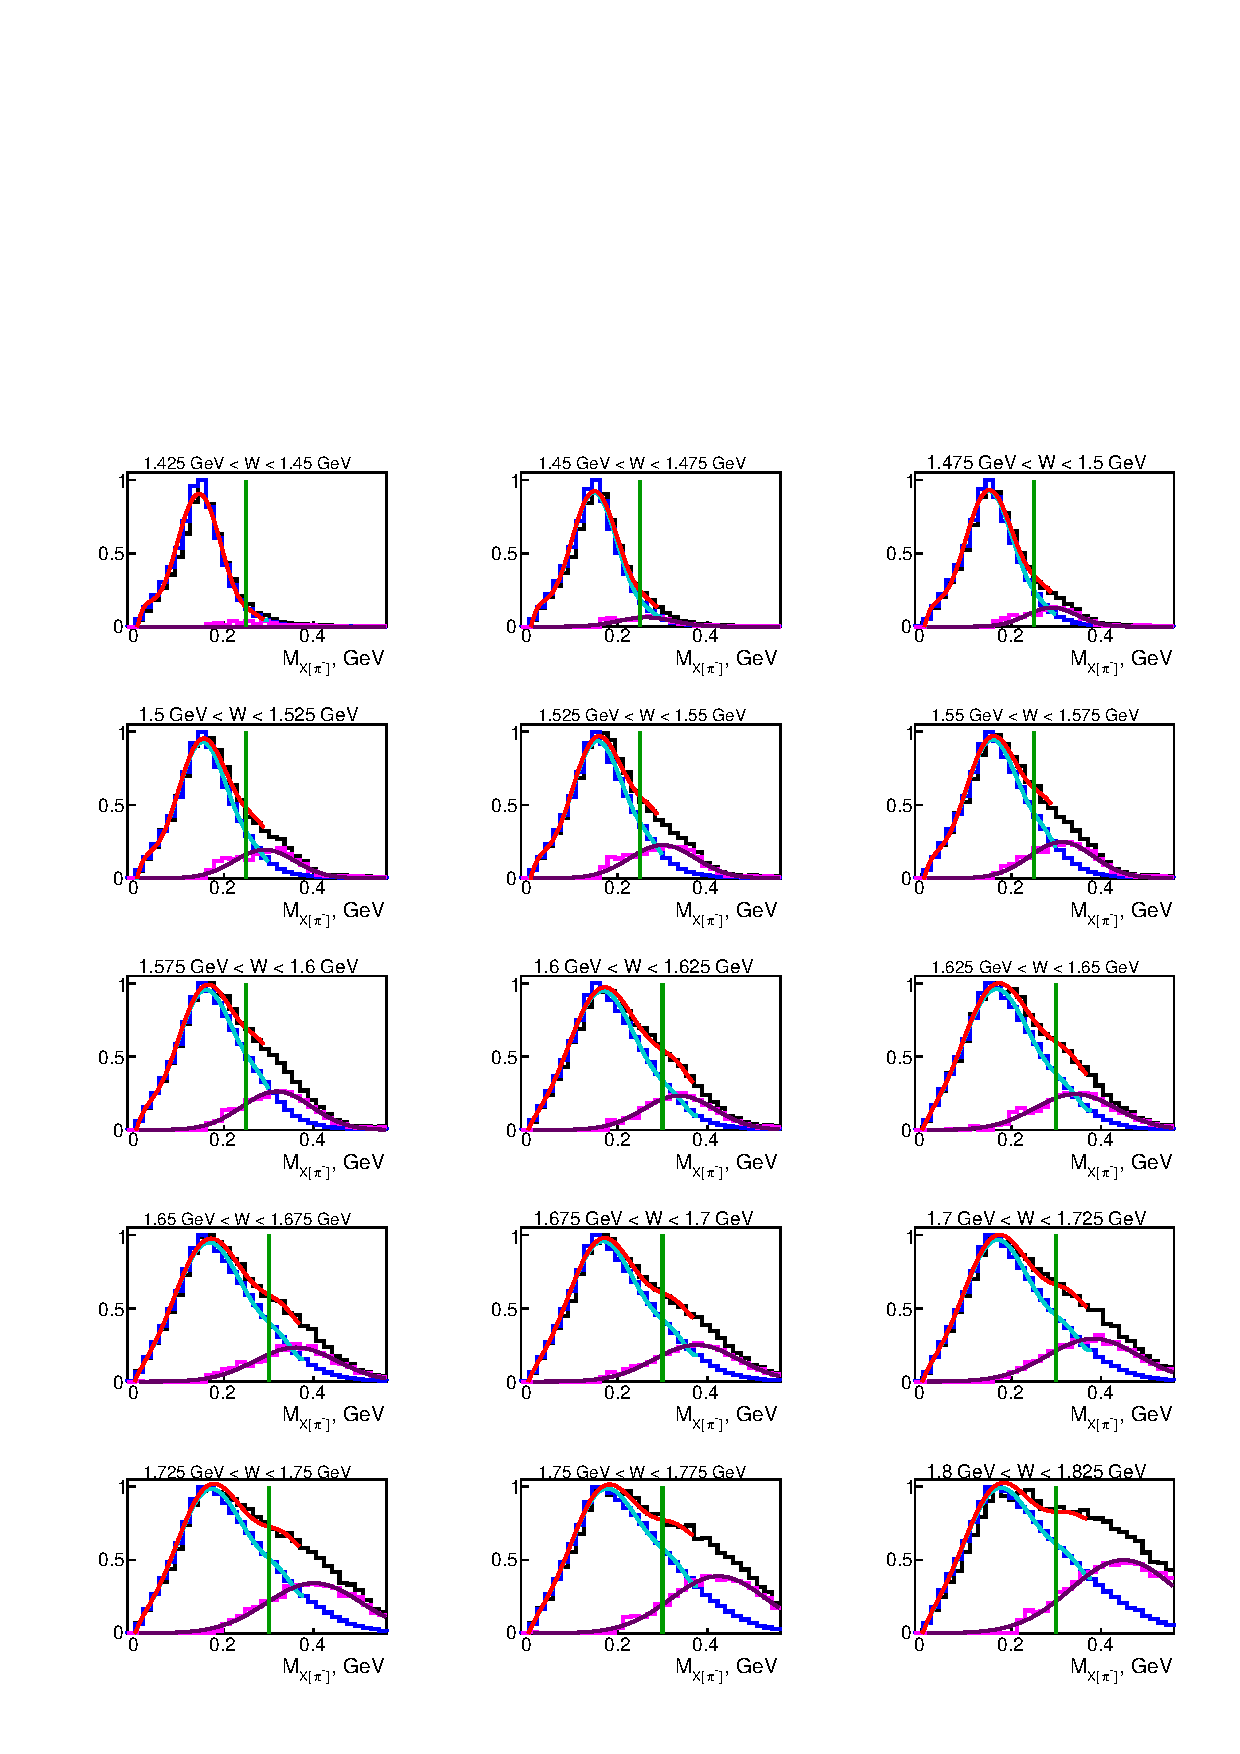
\includegraphics[width=\textwidth]{pictures/other_cuts/excl_cut/main_top_mm_fsi_corr2.pdf}}
\end{center}
\caption{\small Distributions of the quantity $M_{X[\pi^{-}]}$ (defined by Eq.~\eqref{eq:main_top_mm_nosq}) in different 25-MeV-wide $W$ bins for the experimental data (black histograms), Monte Carlo simulation (blue histograms), and their difference (magenta histograms). The explanation of the fit curves is given in the text. Green vertical lines correspond to the position of the cut that is intended to select quasi-free events. The cut is applied to the reconstructed Monte Carlo events as~well.}
\label{fig:main_top_mm_fsi_corr}
\end{figure}
\clearpage


\begin{itemize}
\item The distributions of $M_{X[\pi^{-}]}$ for the reconstructed Monte Carlo events (blue histograms) were fit by a ninth order polynomial in a slightly wider range than marked by the green cut lines. The results of the fit are shown in Fig.~\ref{fig:main_top_mm_fsi_corr} by the cyan curves.
\item The magenta background distributions were fit by Gaussians. The results of the fit are shown by the dark-magenta curves.
\item The cyan and dark-magenta curves were summed up to produce the red curve, which perfectly matches the black experimental histogram in each $W$ bin.
\item The correction factor $F_{fsi}$ was determined in the left side of the green cut~line,
\begin{equation}
 F_{fsi}(W) = \frac{area~under~the~cyan~curve}{area~under~the~red~curve} \leq 1.\label{eq:fsi_corr_fact}
\end{equation}\label{eq:fsi_corr}\vspace{-3em}
\item In each $W$ bin the experimental event yield in the $\pi^{-}$-missing topology is multiplied by the factor $F_{fsi}$, which serves as an effective correction due to the remaining admixture of the FSI-background events.
\end{itemize}


The factor $F_{fsi}$ is assumed to be only $W$ dependent as it was found that it does not demonstrate any $Q^{2}$ dependence, and the dependence on the final hadron variables is neglected due to the statistics limitation. The value of $F_{fsi}$ varies from $\sim$0.97 to $\sim$0.93 in the $W$ range from 1.4625~GeV to 1.8125~GeV, while for $W < 1.4625$~GeV $F_{fsi}=1$ as the correction there is not needed.


Note that the exclusivity cut shown in Fig.~\ref{fig:main_top_mm_fsi_corr} accompanied by the corresponding correction cares for all other possible effects that along with the FSI effects may contribute to the mismatch between the data and the simulation in this topology (including the three-pion background).

